\documentclass[journal]{IEEEtran}

\usepackage{cite}
\usepackage{amsmath,amssymb,amsfonts}
\usepackage{graphicx}
\usepackage{textcomp}
\usepackage{xcolor}
\usepackage{booktabs}
\usepackage{array}
\usepackage{url}
\usepackage[caption=false,font=footnotesize]{subfig}
\usepackage{tikz}
\usepackage{pgfplots}
\pgfplotsset{compat=1.16}
\usetikzlibrary{shapes.geometric,arrows.meta,positioning,calc,fit,backgrounds}
\graphicspath{{figs/}}

% --- Flowchart node styles (compact, IEEE-column friendly) -------------------
\tikzset{
  fcstart/.style={rectangle, rounded corners=6pt, draw, fill=blue!8,
    align=center, font=\scriptsize, minimum height=5mm, inner sep=3pt},
  fcproc/.style={rectangle, draw, fill=gray!6, align=center,
    font=\scriptsize, minimum height=5mm, inner sep=3pt},
  fcdec/.style={diamond, aspect=2, draw, fill=orange!12, align=center,
    font=\scriptsize, inner sep=1pt},
  fcio/.style={trapezium, trapezium left angle=70, trapezium right angle=110,
    draw, fill=green!8, align=center, font=\scriptsize, inner sep=3pt},
  fcarrow/.style={-{Latex[length=2mm]}, thick},
  fclabel/.style={font=\scriptsize\itshape}
}

\def\BibTeX{{\rm B\kern-.05em{\sc i\kern-.025em b}\kern-.08em
    T\kern-.1667em\lower.7ex\hbox{E}\kern-.125emX}}

\begin{document}

\title{A Unified Hybrid Aerial--Aquatic Swarm Architecture\\
Integrating Biomimetic Locomotion, Hierarchical\\
Path Planning, and an Adaptive Cross-Domain\\
Communication Protocol}

\author{I~Harihara~Sudar,
        Mervin~Joe~Thomas,
        Chinmay~K,
        Nanigiri~Laxmi~Narayana~Charan,
        Rishi,
        and~Harsh~Soni%
\thanks{Manuscript prepared June~2026.}%
\thanks{The authors are with the Robotics Lab, Department of Mechanical
Engineering, National Institute of Technology Karnataka (NITK), Surathkal,
India.}%
\thanks{Corresponding author: Mervin~Joe~Thomas
(e-mail: mervinthomas@nitk.edu.in).}}

\markboth{Unified Hybrid Aerial--Aquatic Swarm Architecture}%
{Sudar \MakeLowercase{\textit{et al.}}: A Unified Hybrid Aerial--Aquatic Swarm Architecture}

\maketitle

\begin{abstract}
Single-medium robots are fundamentally constrained: aerial drones offer rapid
mobility and wide situational awareness but cannot sense beneath the surface,
while aquatic robots offer endurance, stealth, and precise underwater
maneuvering but suffer from slow, latency-bound communication and difficult
surface transitions. This paper presents a \emph{unified hybrid aerial--aquatic
swarm architecture} that couples a school of biomimetic robotic fish with a
team of autonomous quadrotors into a single, cooperative, cross-domain system.
The architecture is organized into five layers---physical modeling, hardware
and actuation, control and coordination, hybrid communication, and
simulation/visualization---and integrates three principal contributions. First,
\emph{biomimetic locomotion}: undulatory propulsion grounded in
Lighthill's elongated-body theory and validated by an Arbitrary
Lagrangian--Eulerian (ALE) moving-mesh computational fluid dynamics (CFD)
study, which shows up to a $10\%$ gain in Froude propulsive efficiency for two
fish swimming in antiphase at $0.4L$ spacing, realized in hardware through an
ESP32-driven central pattern generator (CPG) with PID closure. Second,
\emph{hierarchical path planning}: a two-level architecture that combines
global Particle Swarm Optimization (PSO) with local Model Predictive Control
(MPC) and feeds the CPG for the fish and a cascaded ArduPilot/optical-flow
stack for the GNSS-denied drone, including a frustum-guided precision docking
and magnetic auto-charging subsystem; we additionally quantify, in a controlled
graph-theoretic formation study over seven agents and five obstacle seeds, that
contracting the dynamic envelope to fish-like values roughly halves
root-mean-square (RMS) jerk while preserving formation accuracy and a $100\%$
success rate. Third, the novel \emph{ADAPTH} (Adaptive Dynamic Aerial--Aquatic
Path-Tracking and Hybridization) protocol, a relay-based, ``wait-and-verify''
cross-domain communication scheme that bridges low-latency RF and
high-latency acoustic links and sustains $85\%$ end-to-end communication
success in noisy conditions. The complete system is validated in ROS2/Gazebo
with RViz visualization and on hardware prototypes, establishing a reproducible
foundation for persistent, multi-domain swarm missions in environmental
monitoring, search and rescue, and coastal surveillance.
\end{abstract}

\begin{IEEEkeywords}
Bio-inspired swarm robotics, hybrid aerial--aquatic systems, biomimetic robotic
fish, central pattern generator, CFD schooling analysis, PSO--MPC path planning,
cross-domain communication, ADAPTH protocol, GNSS-denied navigation, precision
docking, ROS2/Gazebo.
\end{IEEEkeywords}

\section{Introduction}
\IEEEPARstart{B}{iological} collectives---fish schools, bird flocks, and
insect swarms---exhibit emergent coordination, energy economy, and resilience
to perturbation that continue to inspire engineered autonomous
systems~\cite{reynolds1987flocks,katz2011inferring}. These natural paradigms
demonstrate that distributed, locally interacting agents can achieve global
objectives---coverage, transport, migration---with robustness that centralized
systems struggle to match. Yet most robotic realizations remain confined to a
single medium.

\subsection{Background and Motivation}
Aerial drones provide rapid mobility and wide situational awareness but are
endurance-limited and blind beneath the surface; aquatic robots offer endurance,
stealth, and fine underwater maneuvering but suffer slow communication and
difficult surface transitions~\cite{berlinger2021implicit,tahir2024aerial,qi2025review}.
Missions such as environmental monitoring, search and rescue, and coastal
surveillance demand capabilities no single domain supplies in
isolation~\cite{quattrini2022multirobot}. A \emph{hybrid aerial--aquatic swarm}
coupling biomimetic robotic fish with aerial drones exploits both: drones provide
awareness and act as mobile relays, while fish provide persistent, stealthy
underwater sensing. The two classes are complementary in their failure modes
too---when the drone is grounded for recharge the submerged team keeps sensing,
and when the acoustic link degrades a surfacing drone restores bandwidth---so a
team designed together rather than bolted together can sustain a mission
indefinitely.

\subsection{Problem Statement}
Despite advances in aerial and aquatic robotics, integrated hybrid swarm
operation remains underexplored. Existing research emphasizes single-domain
models, simplified dynamics, or isolated prototypes, leaving gaps in
(i)~hydrodynamic interactions for energy-efficient underwater schooling;
(ii)~unified models capturing aero--hydrodynamic transitions; (iii)~reliable
cross-domain communication and coordination; and (iv)~adaptive control for
stable medium shifts. Realizing the integrated system raises three tightly
coupled challenges:
\begin{itemize}
  \item \textbf{Dynamic heterogeneity.} The team must reconcile aerodynamic
  forces (lift, drag, rotor thrust) with hydrodynamic effects (buoyancy, added
  mass, vortex interactions, drag-limited undulatory thrust) within a single
  planning and control framework.
  \item \textbf{Cross-medium communication.} Air and water are
  electromagnetically incompatible channels: aerial RF links are low-latency and
  high-bandwidth, whereas underwater acoustic links are high-latency
  ($0.5$--$2$~s) and low-bandwidth~\cite{pompili2009underwater,li2023rf}.
  Bridging them reliably requires medium translation and a latency-tolerant
  handshake.
  \item \textbf{Robust swarm coordination.} Distributed control must hold under
  noise, latency, and environmental variability while preserving formation and
  safety.
\end{itemize}

\subsection{Objectives and Approach}
The work develops dynamic models for both agents; a CFD analysis of schooling
thrust and efficiency; validated actuation (CPG tail drive, rotor propulsion) and
integrated sensing/compute hardware; CPG/PID control with hierarchical PSO--MPC
planning and swarm coordination; and the ADAPTH cross-domain protocol. The
end-to-end methodology---modeling, CFD, actuation, hardware, planning, ADAPTH, and
ROS2/RViz validation---is summarized as a flowchart in Fig.~\ref{fig:method}.

\begin{figure}[!t]
\centering
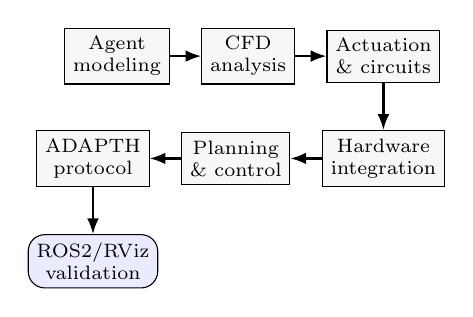
\begin{tikzpicture}[node distance=2.6mm and 4mm]
\node[fcproc] (m1) {Agent\\modeling};
\node[fcproc, right=of m1] (m2) {CFD\\analysis};
\node[fcproc, right=of m2] (m3) {Actuation\\\& circuits};
\node[fcproc, below=6mm of m3] (m4) {Hardware\\integration};
\node[fcproc, left=of m4] (m5) {Planning\\\& control};
\node[fcproc, left=of m5] (m6) {ADAPTH\\protocol};
\node[fcstart, below=6mm of m6] (m7) {ROS2/RViz\\validation};
\draw[fcarrow] (m1)--(m2); \draw[fcarrow] (m2)--(m3);
\draw[fcarrow] (m3)--(m4); \draw[fcarrow] (m4)--(m5);
\draw[fcarrow] (m5)--(m6); \draw[fcarrow] (m6)--(m7);
\end{tikzpicture}
\caption{Methodological framework integrating modeling, CFD, actuation, hardware,
planning, the ADAPTH communication protocol, and ROS2/RViz validation.}
\label{fig:method}
\end{figure}

\subsection{Contributions and Scope}
This work makes three principal contributions, each developed in a dedicated
section: a \emph{biomimetic-locomotion subsystem} validated by CFD and realized
in CPG hardware (Section~\ref{sec:locomotion}); a \emph{hierarchical
path-planning and GNSS-denied navigation framework} with precision docking,
benchmarked by a controlled graph-theoretic formation study
(Sections~\ref{sec:aerial}--\ref{sec:planning}); and the novel \emph{ADAPTH}
cross-domain communication protocol (Section~\ref{sec:adapth}). We are explicit
about fidelity: hydrodynamic gains are established in CFD and bench/water tests;
the swarm-formation study uses a second-order SO(3) agent model with a contracted
dynamic envelope rather than a full hydrodynamic, non-holonomic swimmer; and
ADAPTH is validated on a relay-based prototype. The system is validated in
simulation and hardware prototypes, with full-scale field deployment left to
future work. The remainder of the paper is organized as
Sections~\ref{sec:related}--\ref{sec:concl}: related work, the five-layer
architecture, biomimetic locomotion, the aerial platform, hierarchical planning,
ADAPTH, consolidated results, discussion, and conclusion.

\section{Related Work}
\label{sec:related}

\subsection{Bio-Inspired Locomotion and Hydrodynamics}
Bio-inspired robotics seeks to emulate the efficiency and robustness of
biological swimmers~\cite{triantafyllou2000hydrodynamics,sfakiotakis1999review}.
Fish-like robots exploit undulatory locomotion---carangiform, anguilliform,
ostraciiform modes---to achieve high thrust efficiency and maneuverability.
Lighthill's large-amplitude elongated-body theory~\cite{lighthill1971large}
remains the foundational model of undulatory propulsion, accounting for reactive
forces, vortex shedding, and added mass; Majeed and Ali~\cite{majeed2014dynamic}
parameterize the body wave with a polynomial amplitude envelope. Schooling
hydrodynamics---energy savings from vortex exploitation and drafting---trace to
Weihs~\cite{weihs1973hydromechanics} and have since been examined in high-fidelity
CFD~\cite{borazjani2008numerical,daghooghi2015hydrodynamic,koca2025comparative,kern2006simulations}.
We build directly on this lineage, using ALE moving-mesh CFD with realistic
kinematics to quantify antiphase schooling gains.

\subsection{Control of Biomimetic Fish}
Rhythmic locomotion is most naturally generated by central pattern generators
(CPGs), networks of coupled nonlinear oscillators that produce stable limit
cycles~\cite{xie2019cpg}; recent work adds fault tolerance~\cite{wang2025fuzzy}
and couples CPGs with MPC for trajectory tracking~\cite{yan2022bionic}.
Iterative learning control refines repeated trajectories~\cite{wang2020iterative},
and data-driven neural models improve dynamic
prediction~\cite{zhong2026datadriven}. Our fish node adopts a CPG--PID cascade
whose references are modulated online by the high-level planner: the CPG's few
parameters (amplitude, frequency, inter-segment phase) form a compact interface
that a planner or remote command can bias without re-deriving a trajectory---the
property exploited by the ADAPTH ``CPG bias'' command---while keeping on-node
computation light enough for a microcontroller.

\subsection{Hybrid Aerial--Aquatic Systems}
Hybrid platforms span folding-wing transitioners, magnetically driven
collectives, dual-mode drones, and multi-modal HAUVs
(Table~\ref{tab:hybrid})~\cite{tahir2024aerial,qi2025review,kim2022swarm,zhang2023rfoptical}.
Blueswarm demonstrates implicit, vision-only 3D coordination in a fish-inspired
underwater swarm~\cite{berlinger2021implicit}. Persistent challenges include
fluid--structure interaction, buoyancy control, and interface communication. Our
system targets the integration gap: a single architecture coupling both agent
classes under one planner and one communication protocol.

\begin{table}[!t]
\centering
\caption{Comparison of Hybrid Aerial--Aquatic Robotic Systems}
\label{tab:hybrid}
\begin{tabular}{p{1.5cm}p{2.2cm}p{2.6cm}}
\toprule
System & Transition mechanism & Key advantage\\
\midrule
AquaMAV       & Folding wings        & Rapid air--water transition\\
Magnebot swarm& Magnetic actuation   & Collective motion\\
Hybrid UAV--AUV& RF--acoustic relay   & Cross-domain comm.\\
Dual-mode drone& Optical--RF switching& Low-latency transfer\\
HAUV          & Multi-modal propulsion& Marine optics\\
\bottomrule
\end{tabular}
\end{table}

\subsection{Swarm Intelligence and Optimization-Based Planning}
Swarm robotics uses local interactions for global
behavior~\cite{reynolds1987flocks}. For dense-clutter formation flight, a line of
optimization-based planners treats each robot's path as a continuous trajectory:
EGO-Swarm~\cite{zhou2021egoswarm} provides a gradient-based, ESDF-free local
planner; MINCO~\cite{wang2022geometrically} supplies a minimum-control polynomial
parameterization; and Swarm-Formation~\cite{quan2022distributed,quan2023robust}
adds a differentiable graph-similarity term so a swarm holds shape through
clutter. At the mission level, Particle Swarm
Optimization~\cite{kennedy1995particle} and Model Predictive
Control~\cite{mayne2000constrained} are widely combined for global--local
planning~\cite{cao2025path,mu2022path,liu2026improved,liu2017planning}.
Table~\ref{tab:coord} contrasts representative coordination strategies; we adopt a
PSO--MPC hierarchy and use the graph-theoretic planner as a controlled testbed.

\begin{table}[!t]
\centering
\caption{Comparison of Swarm Coordination Algorithms}
\label{tab:coord}
\begin{tabular}{p{1.5cm}p{2.0cm}p{1.4cm}p{1.4cm}}
\toprule
Algorithm & Principle & Strength & Limitation\\
\midrule
Boids    & Rule-based flocking & Simple patterns & Disturbance-sensitive\\
PSO      & Social optimization & Convergence     & Local minima\\
MPC      & Predictive control  & Optimal paths   & Compute cost\\
PSO--MPC & Hybrid optimization & Efficiency      & Tuning effort\\
\bottomrule
\end{tabular}
\end{table}

\subsection{Cross-Domain Communication}
The persistent bottleneck for hybrid teams is communication across the air--water
boundary. Underwater acoustic networks are slow and
bandwidth-limited~\cite{pompili2009underwater}; aerial swarms use RF
meshes~\cite{li2023rf}; hybrids rely on surface
relays~\cite{quattrini2022multirobot} or optical inter-domain
links~\cite{zhang2023rfoptical}, and recent protocols add trust and cryptographic
guarantees~\cite{singh2025simulation}. Table~\ref{tab:comm} contrasts the dominant
modalities. Existing protocols rarely provide an adaptive, mission-prioritized
handshake spanning both media---the gap ADAPTH targets.

\begin{table}[!t]
\centering
\caption{Comparison of Communication Modalities}
\label{tab:comm}
\begin{tabular}{lccc}
\toprule
Medium & Latency & Range & Environment\\
\midrule
RF              & $10$--$100$~ms  & $1$--$5$~km  & Air\\
Acoustic        & $0.5$--$2$~s    & $1$--$2$~km  & Water\\
Optical         & $50$--$200$~ms  & $10$--$100$~m & Water/surface\\
Hybrid RF--Acoustic & $100$--$500$~ms & up to $2$~km & Interface\\
\bottomrule
\end{tabular}
\end{table}

\section{Unified System Architecture}
\label{sec:arch}
The hybrid swarm integrates physical modeling, hydro/aerodynamic analysis,
multi-agent coordination, hybrid communication, actuation, hardware
prototyping, and visualization into a single framework structured as five
interconnected layers:
\begin{enumerate}
  \item \textbf{Physical modeling layer.} Hydrodynamic models for the fish
  (Lighthill EBT~\cite{lighthill1971large}, polynomial body
  wave~\cite{majeed2014dynamic}, added mass, wake, schooling) validated by CFD,
  and Newton--Euler rotor dynamics for the drone with bio-inspired stability.
  \item \textbf{Hardware and actuation layer.} ESP32 + IMU + magnetometer +
  DC/BLDC tail actuation for the fish; Pixhawk + Raspberry~Pi~5 + BLDC/ESC for
  the drone (Table~\ref{tab:hw}).
  \item \textbf{Control and coordination layer.} CPG/PID and ILC for fish,
  cascaded PID/MPC for the drone, and PSO--MPC with Boids-style interaction for
  the swarm, ensuring collision avoidance and formation adaptability.
  \item \textbf{Hybrid communication layer.} Aerial RF mesh and underwater
  acoustics bridged by a surface relay, carrying ADAPTH packets for routing and
  handshakes, with optical channels enhancing interface transfers.
  \item \textbf{Simulation and visualization layer.} MATLAB/Simulink for
  dynamics and actuation, ANSYS Fluent for CFD, and ROS2/Gazebo with RViz for
  multi-agent visualization, incorporating hardware data for realism.
\end{enumerate}

\begin{table}[!t]
\centering
\caption{Hardware Components Overview}
\label{tab:hw}
\begin{tabular}{lll}
\toprule
Agent & Component & Function\\
\midrule
Fish  & ESP32                & Control and PWM generation\\
      & IMU / magnetometer   & Orientation / heading\\
      & DC / BLDC motors     & Tail / fin actuation\\
\midrule
Drone & Raspberry~Pi~5       & High-level planning, perception\\
      & Pixhawk              & Flight stabilization\\
      & GPS / camera / LiDAR & Positioning, tracking, mapping\\
\bottomrule
\end{tabular}
\end{table}

A dedicated transition controller, embedded in the ADAPTH layer, links the
domains. A \emph{medium-inference} block fuses sensor data to detect the operating
environment; a \emph{dynamics switcher} selects the aero- or hydro-dynamic model;
a \emph{controller bank} activates PID/MPC/CPG as appropriate; a
\emph{coordination engine} maintains cross-domain formations; and a
\emph{latency-aware planning module} schedules paths against the available link
budget. Prototyped on a Raspberry~Pi~5 aerial node and an ESP32 aquatic node, this
transition layer achieves $85\%$ communication success during cross-domain
operation.

\section{Biomimetic Locomotion and Hydrodynamic Modeling}
\label{sec:locomotion}

\subsection{Undulatory Propulsion Model}
Following Lighthill~\cite{lighthill1971large} and the polynomial envelope of
Majeed and Ali~\cite{majeed2014dynamic}, the lateral displacement of the fish
body at longitudinal coordinate $x$ and time $t$ is
\begin{equation}
y(x,t) = \big(a_0 + a_1 x + a_2 x^2\big)\sin(2\pi f t + k x),
\label{eq:bodywave}
\end{equation}
where $a_0,a_1,a_2$ shape the amplitude envelope, $f$ is the tail-beat
frequency, and $k=2\pi/\lambda$ is the body wavenumber. The reactive thrust and
lateral hydrodynamic force follow as
\begin{equation}
T = \rho S\!\left(U\frac{\partial y}{\partial t}
   - \tfrac{1}{2}U^2\frac{\partial y}{\partial x}\right),
\qquad
F_y = \rho S\,\frac{\partial^2 y}{\partial t^2},
\label{eq:thrust}
\end{equation}
with water density $\rho$, effective body surface area $S$, and forward
swimming speed $U$. These expressions provide the closed-form thrust/drag/lateral
forces used for control design and are corroborated by the CFD study below.

\subsection{Computational Fluid Dynamics}
To quantify the energetic benefit of schooling, we performed an ALE moving-mesh
CFD study in ANSYS Fluent 2025~R1 using realistic body undulation rather than an
idealized sinusoid. The pipeline comprised CAD simplification, meshing,
convergence verification, and a spacing/phasing parameter sweep.

\subsubsection{CAD Geometry and Simplification}
The robotic fish was designed as a laterally compressed, carangiform body with a
lunate caudal fin, paired pectoral and dorsal fins, and a segmented posterior
section housing the actuation linkage (Fig.~\ref{fig:fishcad}). The original CAD
geometry was simplified before meshing: non-essential surface features that
minimally affect the pressure distribution governing lift and drag were removed,
reducing cell count while preserving the key hydrodynamic physics and improving
mesh quality and numerical stability~\cite{borazjani2008numerical}. The body
length is $L=43.9$~cm.

\begin{figure}[!t]
\centering
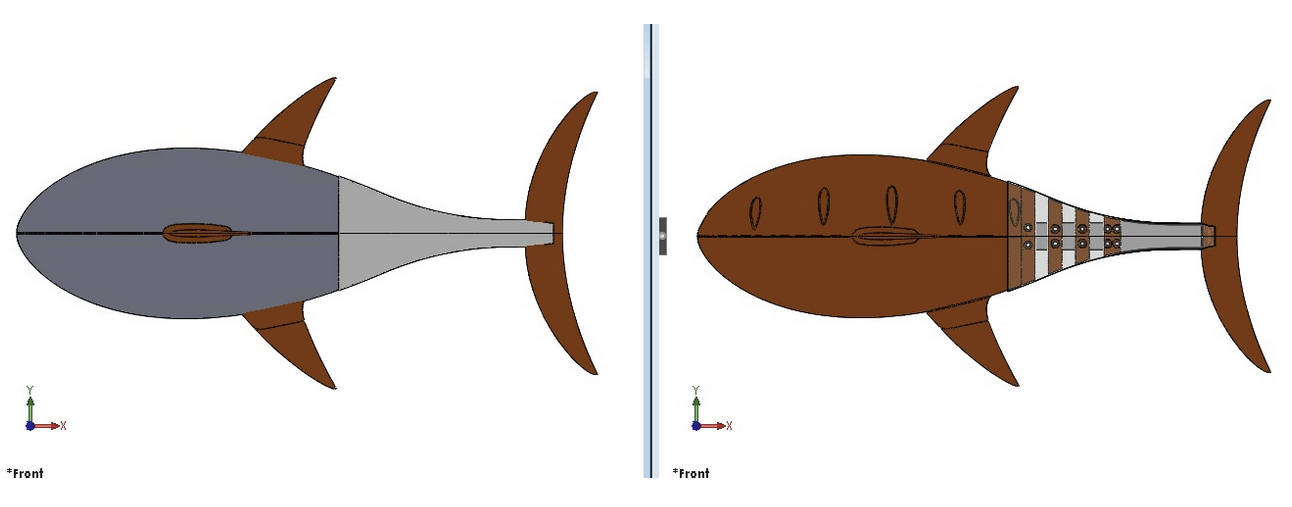
\includegraphics[width=\columnwidth]{fish_cad.png}
\caption{CAD model of the biomimetic robotic fish (front views): a laterally
compressed carangiform body with lunate caudal fin, dorsal and pectoral fins, and
a segmented posterior section (right) housing the multi-link tail actuation.
The nose is aligned along $+x$.}
\label{fig:fishcad}
\end{figure}

\subsubsection{Meshing Strategy}
A hybrid tetrahedral mesh with prism inflation layers resolved the boundary
layer. For the solo fish, the mesh ranged $2$--$64$~mm with a $2$~mm near-body
size and three inflation layers (first layer $0.4$~mm, growth rate $1.0$),
totaling $\sim\!1.2$~million cells. For the parallel-fish case the mesh was
refined to a $2$--$32$~mm range, $4$~mm near-body sizing, and eight inflation
layers (first layer $0.8$~mm, growth rate $1.1$), with overlapping multi-region
meshes handling the two independent bodies. The resulting hybrid mesh
(Fig.~\ref{fig:fishmesh}) comprised $\sim\!5.27$~million nodes and a mix of
polyhedral, quadrangle, and triangular cells, meeting orthogonality and skewness
quality criteria. Tables~\ref{tab:cfd1} and~\ref{tab:cfd2} summarize the flow
conditions and solver setup.

\begin{figure}[!t]
\centering
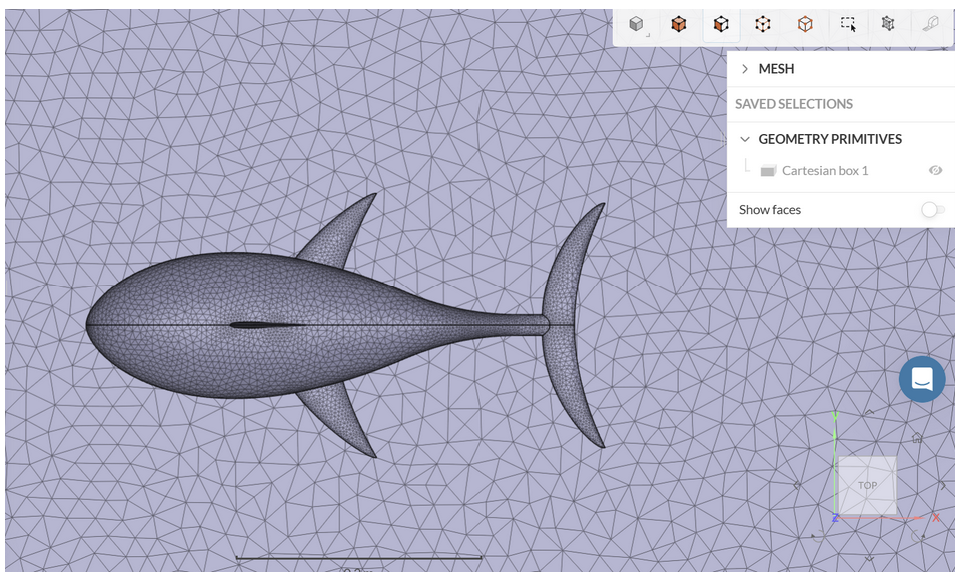
\includegraphics[width=0.9\columnwidth]{fish_mesh.png}
\caption{Hybrid tetrahedral mesh with prism inflation layers around the fish body,
refined near the surface to resolve the boundary layer and the near-wake.}
\label{fig:fishmesh}
\end{figure}

\subsubsection{Mesh Convergence}
Convergence was assessed by monitoring residuals---imbalances in the discretized
Navier--Stokes equations---alongside the physical force histories. A monotone
decreasing residual trend together with stable drag and thrust confirmed solution
reliability; simulations were iterated until residuals fell below
$10^{-4}$~\cite{versteeg2007introduction}.

\subsubsection{Simulation Setup and Results}
The incompressible Navier--Stokes equations were solved with a finite-volume
method, body motion handled by the ALE formulation, and turbulence closed with
the AKN $k$--$\epsilon$ model, suitable for the low-Reynolds, undulating-body
regime. Five forward speeds ($U_x \approx 0.42$--$0.83$~m/s) spanned the Reynolds
range. Forces were obtained by integrating pressure and viscous shear over the
body, and propulsive performance was evaluated through the Froude efficiency
\begin{equation}
\eta = \frac{P_T}{P_T + P_S},
\label{eq:froude}
\end{equation}
where $P_T$ is useful thrust power and $P_S$ is lateral (side-force) power.
Across the spacing/phasing sweep, \emph{antiphase} synchronization at the closest
$0.4L$ spacing produced the strongest constructive wake interaction and up to a
$10\%$ Froude-efficiency gain over solitary swimming, consistent with the
vortex-exploitation mechanism of
schooling~\cite{weihs1973hydromechanics,daghooghi2015hydrodynamic}. Efficiency
improved monotonically as spacing tightened from $2.0L$ to $0.4L$, with the
Strouhal number rising from the solitary optimum $St\!\approx\!0.34$ to
$0.42$--$0.44$ in the parallel cases. The energetic incentive thus grows as the
school tightens, motivating the close, phase-coordinated hexagon used in the swarm
study (Section~\ref{sec:planning}). The velocity field (Fig.~\ref{fig:fishvel})
shows accelerated flow over the body, nose stagnation, and the structured caudal
wake whose constructive overlap underlies the gain.

\begin{figure}[!t]
\centering
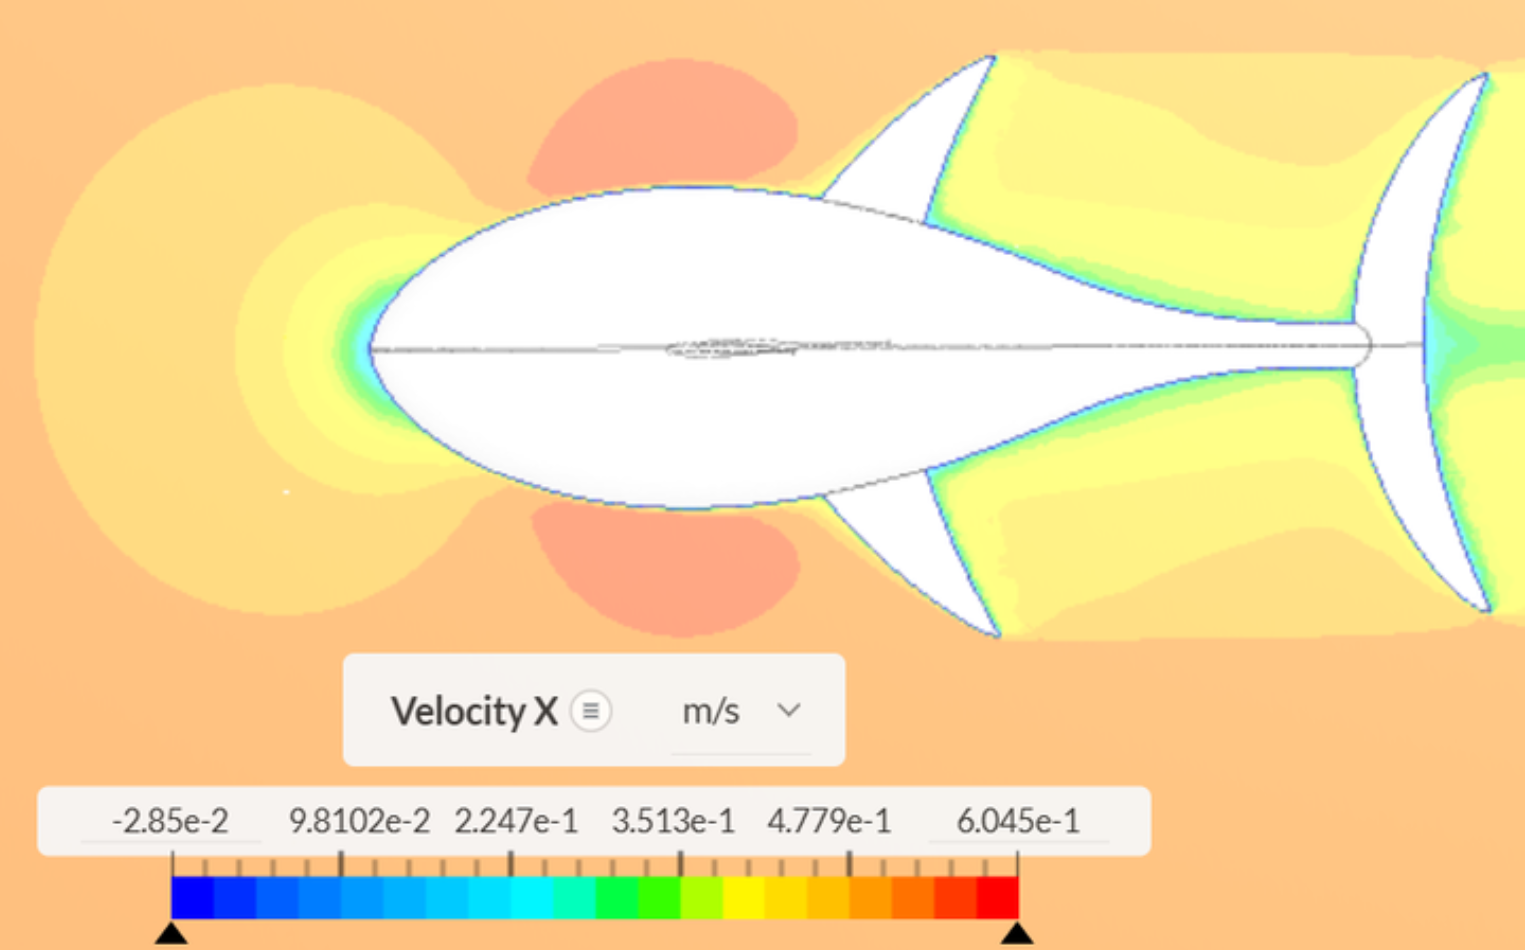
\includegraphics[width=\columnwidth]{fish_velocity.png}
\caption{Streamwise velocity ($V_x$, m/s) contour around the undulating fish from
the ALE moving-mesh CFD: accelerated flow over the body, nose stagnation, and the
caudal wake that drives schooling efficiency when constructively shared between
neighbors.}
\label{fig:fishvel}
\end{figure}

\begin{table}[!t]
\centering
\caption{Flow Conditions and CFD Setup}
\label{tab:cfd1}
\begin{tabular}{ll}
\toprule
Parameter & Specification\\
\midrule
Fluid                 & Water @ $20^\circ$C\\
Density $\rho$        & $998$~kg/m$^3$\\
Flow speeds tested    & $1.01$--$2.02$~BL/s\\
Reynolds number       & $\sim\!2.6\times10^{5}$\\
Strouhal (solo)       & $0.34$\\
Strouhal (parallel)   & $0.42$--$0.44$\\
Domain (solo)         & $5.0L\times4.0L\times2.0L$\\
Fish surface          & Moving wall (no-slip)\\
\bottomrule
\end{tabular}
\end{table}

\begin{table}[!t]
\centering
\caption{Mesh and Solver Details}
\label{tab:cfd2}
\begin{tabular}{ll}
\toprule
Category & Specification\\
\midrule
Mesh type            & Tetrahedral + prism layers\\
Solver               & FV incompressible Navier--Stokes\\
Software             & ANSYS Fluent 2025~R1\\
Body motion          & ALE (Arbitrary Lagrangian--Eulerian)\\
Two-fish handling    & Overlapping / multi-region mesh\\
Turbulence model     & AKN $k$--$\epsilon$\\
Spacings tested      & $0.4L$, $0.6L$, $0.8L$, $1.2L$, $1.6L$, $2.0L$\\
Tail phasing         & In-phase and antiphase\\
\bottomrule
\end{tabular}
\end{table}

\subsection{Fish Node: Actuation and Control}
The locomotion model is realized on an ESP32-based fish node whose complete
actuation and sensing circuit is shown in Fig.~\ref{fig:fishcircuit}. The caudal
tail is driven by a DC motor through an L293D H-bridge; the ESP32 generates the
PWM and closes the loop on MPU6050 IMU and LIS2MDL magnetometer feedback fused
over I$^2$C (with Kalman filtering for noise reduction). Power is supplied by a
3S LiPo regulated to a clean $5$~V logic rail by an LM2596 buck converter, and all
sections share a common ground bus to avoid driver-induced reference offsets.

\begin{figure}[!t]
\centering
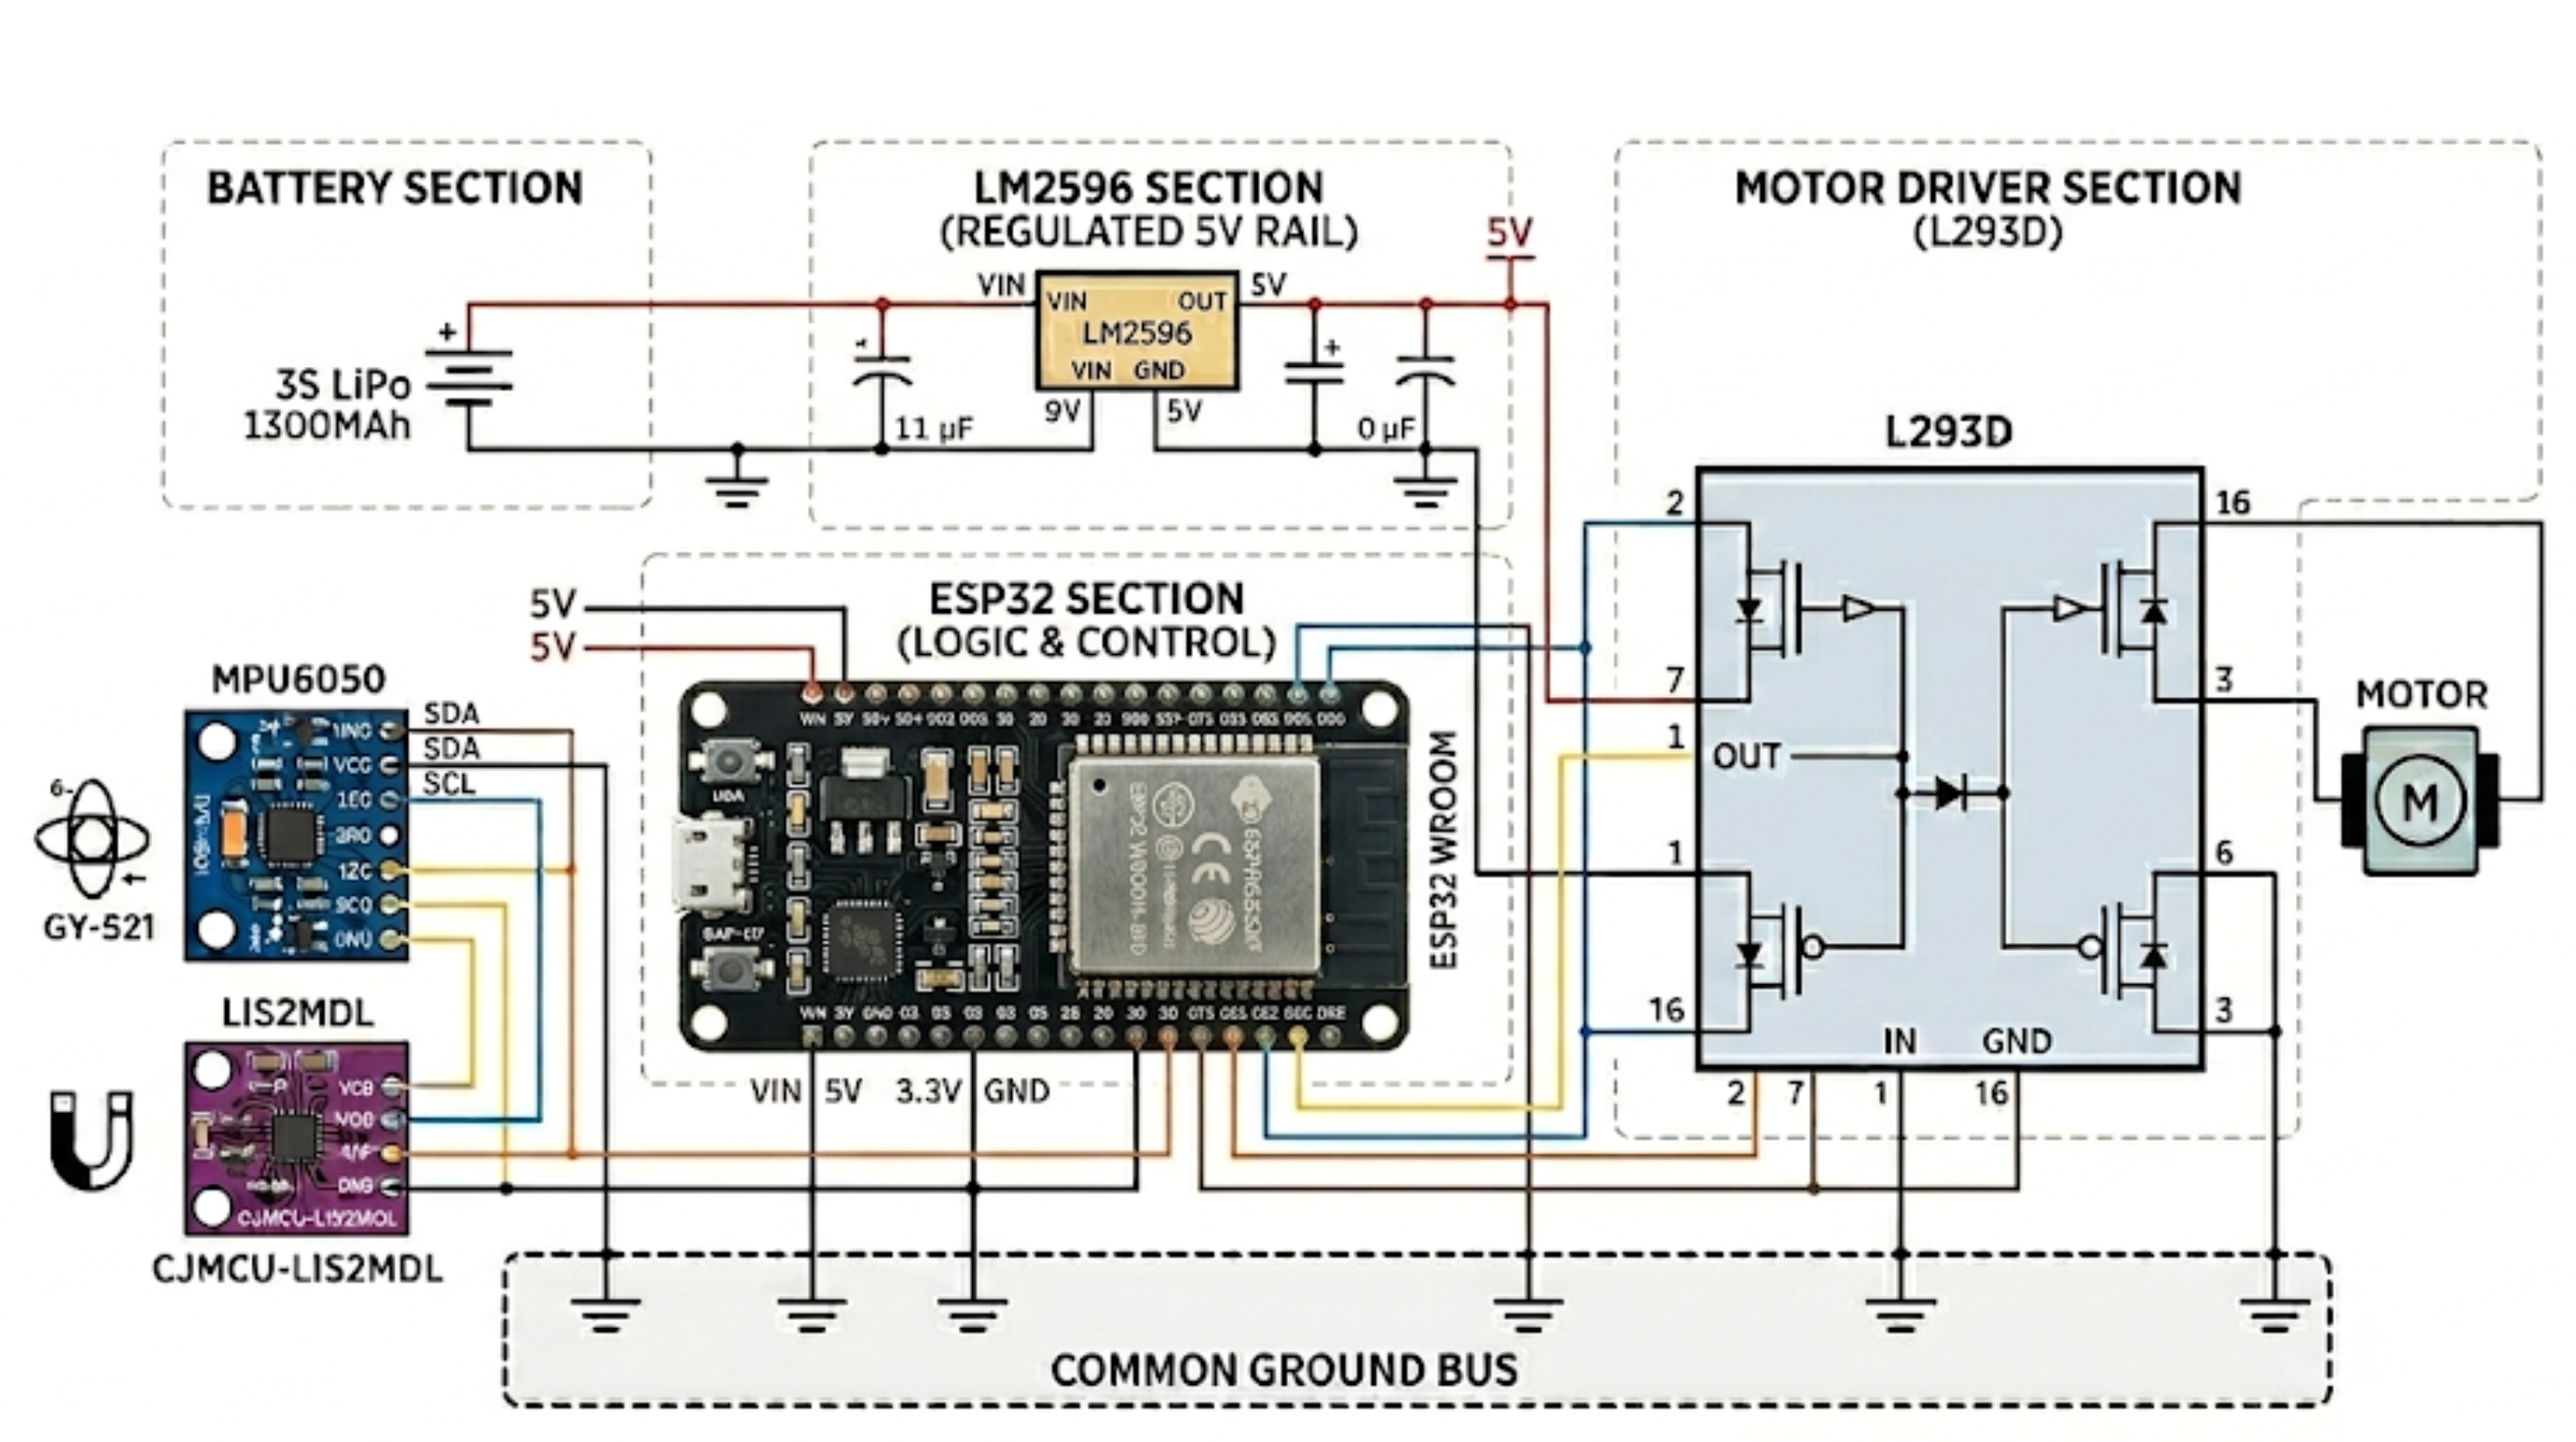
\includegraphics[width=\columnwidth]{fish_circuit.png}
\caption{Robotic-fish actuation and sensing circuit: a 3S LiPo feeds an LM2596
$5$~V regulated rail; the ESP32 reads the MPU6050 IMU and LIS2MDL magnetometer over
I$^2$C and drives the tail DC motor through an L293D H-bridge over a common
ground bus.}
\label{fig:fishcircuit}
\end{figure}

\subsubsection{DC Motor Dynamics}
The motor obeys the standard electromechanical relations
\begin{equation}
V = IR + L\frac{dI}{dt} + K_e\omega,
\qquad
\tau = K_t I = J\frac{d\omega}{dt} + b\omega + \tau_L,
\label{eq:dcmotor}
\end{equation}
with armature current $I$, resistance $R$, inductance $L$, back-EMF constant
$K_e$, torque constant $K_t$, inertia $J$, viscous friction $b$, and a load
torque $\tau_L$ supplied by the hydrodynamic forces of \eqref{eq:thrust}. The
effective drive voltage is $V_{\mathrm{eff}}=D\,V_{\mathrm{supply}}$ for duty
cycle $D$, and the H-bridge enables bidirectional (oscillatory) tail motion.

\subsubsection{CPG and PID Control}
Rhythmic references come from a CPG modeled as coupled nonlinear oscillators,
\begin{equation}
\ddot{\theta}_i + \alpha\big(\theta_i^2 + \dot{\theta}_i^2 - A^2\big)\dot{\theta}_i
+ \omega^2\theta_i = \sum_{j} w_{ij}\,(\theta_j - \theta_i),
\label{eq:cpg}
\end{equation}
whose limit-cycle amplitude $A$ and frequency $\omega$ are modulated online by
the high-level planner, and whose inter-oscillator coupling $w_{ij}$ sets the
inter-segment phase for multi-segment tails. A PID law tracks the CPG reference
$\theta_d$,
\begin{equation}
u(t) = K_p\,e(t) + K_i\!\int_0^t\! e(\tau)\,d\tau + K_d\,\frac{d\,e(t)}{dt},
\qquad e=\theta_d-\theta,
\label{eq:pid}
\end{equation}
and is tuned to limit overshoot and settling time. The working cycle is:
sensors estimate orientation/heading; the CPG generates the rhythmic beat
pattern; the PID computes a corrective PWM from the CPG--sensor error; the H-bridge
drives the motor; and current limiting plus emergency stop protect against
burnout. The loop responds in under $10$~ms.

\subsubsection{Simulink Validation and Degrees of Freedom}
The actuation system was modeled in MATLAB/Simulink (Simscape Electrical) with
CFD-derived hydrodynamic loads applied as variable torques. Step-response and
sinusoidal-tracking tests give a rise time below $0.5$~s, steady-state error
under $5\%$, and an average cruise power near $5$~W. A multi-segment tail adds
degrees of freedom through phase-delayed oscillation,
$\theta_i(t)=A_i\sin(\omega t + \phi_i)$, enabling curved paths and sharp turns
for swarm avoidance and formation change. Integrated into the swarm simulation,
coordinated (schooling) actuation reduced simulated group energy use by $\sim\!20\%$,
and the hardware node held heading error below $5\%$ in controlled water tests.

The DC caudal drive was chosen for its high low-speed torque, low cost, and easy
PWM control; back-EMF and heating are managed through driver selection and current
limiting. Kalman-filtered IMU/magnetometer fusion rejects driver-induced noise for
a stable PID inner loop. The coupling is bidirectional: fish tail frequency and
amplitude feed the CFD hydrodynamic model, while ADAPTH coordination commands
adjust the CPG parameters, so the $10\%$ efficiency incentive expresses itself as a
controllable formation rather than a static analysis result.

\section{Aerial Platform: Mechanical Design, GNSS-Denied Navigation, and Precision Docking}
\label{sec:aerial}
The aerial agent is an autonomous quadrotor built for GNSS-denied operation, with
a base station that provides precision docking and autonomous recharge while
doubling as the ADAPTH communication gateway. The assembled airframe is shown in
the CAD views of Fig.~\ref{fig:vehicle} and the integrated flight prototype---with
companion computer, downward camera/gimbal, LiDAR, and propeller guards---in
Fig.~\ref{fig:dronephoto}.

\begin{figure}[!t]
\centering
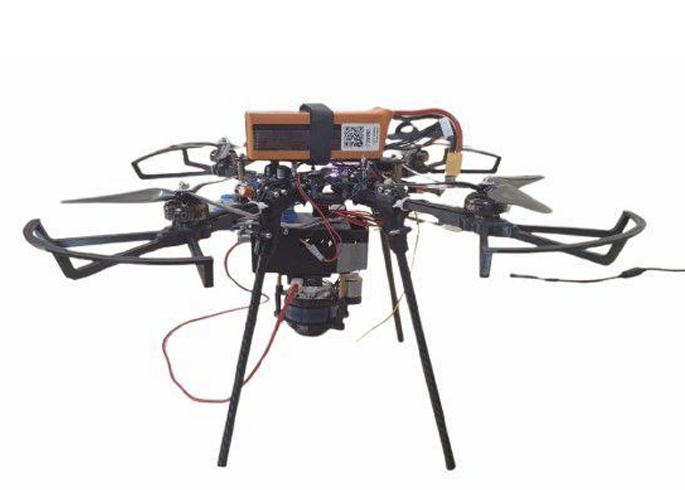
\includegraphics[width=0.78\columnwidth]{drone_photo.png}
\caption{Integrated quadrotor flight prototype: carbon-fiber frame with splayed
landing legs, companion computer and battery on the top plate, downward
camera/gimbal and 1D/2D LiDAR beneath, and full-perimeter propeller guards.}
\label{fig:dronephoto}
\end{figure}

\begin{figure}[!t]
\centering
\subfloat[Front view]{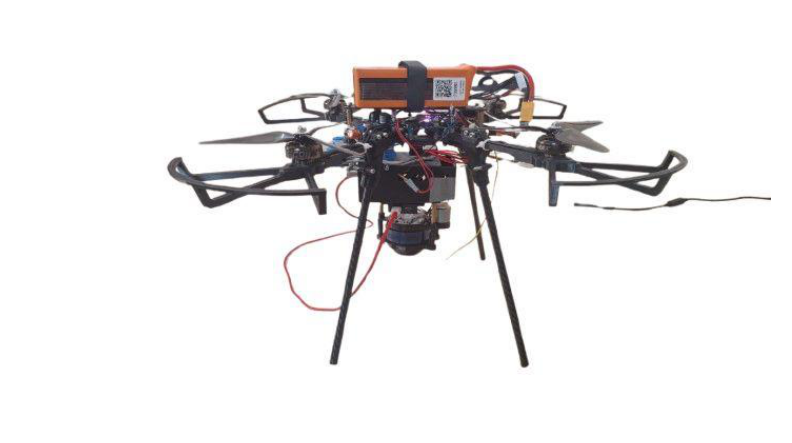
\includegraphics[width=0.52\columnwidth]{fig02a_front.png}}
\hfil
\subfloat[Top view]{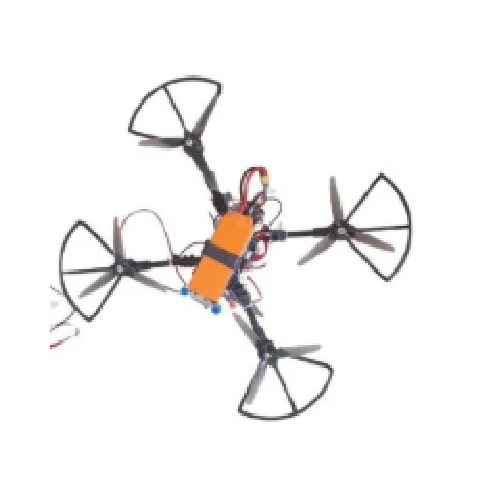
\includegraphics[width=0.40\columnwidth]{fig02b_top.png}}
\caption{The quadrotor airframe with integrated downward LiDAR, global-shutter
camera, and companion computer.}
\label{fig:vehicle}
\end{figure}

\subsection{Mechanical Design}

\subsubsection{Docking Frustum}
Terminal recovery relies on a passively self-aligning, funnel-shaped (frustum)
landing structure (Table~\ref{tab:frustum}). During descent the UAV uses optical
flow and HSV masking to localize the landing area; the frustum geometry then
mechanically corrects residual lateral error, guiding the vehicle to the geometric
center. A $200$~mm radial clearance between propeller tips and the inner cone
yields a $50.67^\circ$ half-angle, and the $1370$~mm outer diameter absorbs landing
inaccuracies. The frustum is fabricated from 18-gauge galvanized iron (GI) for a
high rigidity-to-weight ratio and reinforced by a modular aluminum-extrusion
framework.

\begin{table}[!t]
\centering
\caption{Frustum Geometry}
\label{tab:frustum}
\begin{tabular}{cccc}
\toprule
Half-angle ($^\circ$) & Outer dia.\ (mm) & Inner dia.\ (mm) & Height (mm)\\
\midrule
$50.67$ & $1370$ & $420$ & $390$\\
\bottomrule
\end{tabular}
\end{table}

\subsubsection{Charging Subsystem}
On touchdown a magnetic coupling mates with onboard copper plates and closes the
charging circuit automatically (Fig.~\ref{fig:charging}). A $300$~W AC--DC
switch-mode supply ($24$~V/$12.5$~A out) charges the 6S LiPo, while a PZEM-051
monitor reports voltage, current, power, and cumulative energy---a reliable proxy
for charge completion. The regulated $\sim\!25.3$~V output passes through a
$0.01~\Omega$ shunt and a voltmeter/ammeter pair before splitting to the base-plate
and cone-frustum electrodes. The landing pad is a circular GI sheet on a
spring mechanism that damps landing energy.

\begin{figure}[!t]
\centering
\subfloat[Charging schematic]{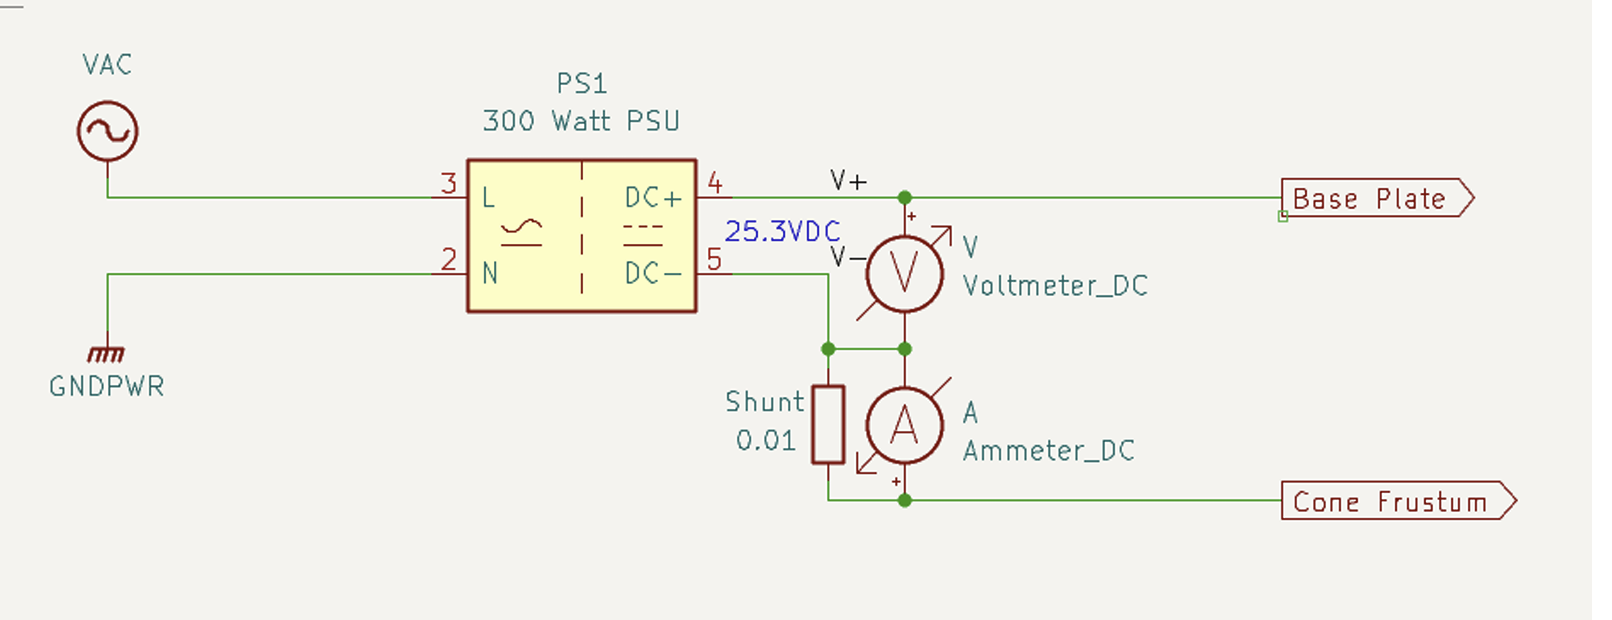
\includegraphics[width=0.56\columnwidth]{bs_circuit.png}}
\hfil
\subfloat[Fabricated landing pad]{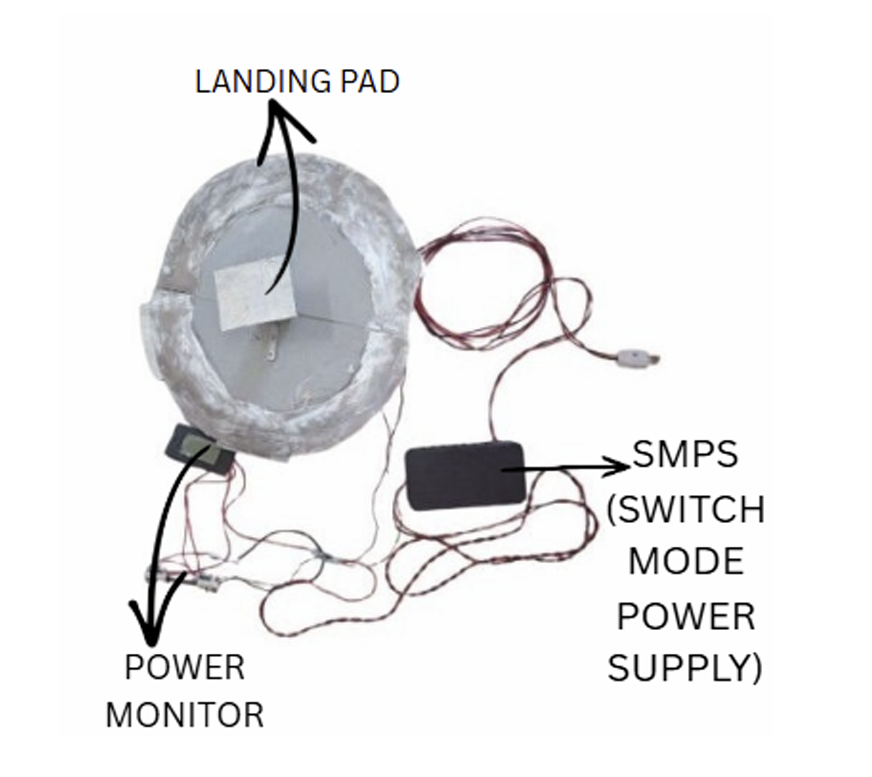
\includegraphics[width=0.40\columnwidth]{landing_pad.png}}
\caption{Base-station charging: (a) the $300$~W supply feeds a shunt and
voltmeter/ammeter before the base-plate and cone-frustum electrodes that close
against the UAV's copper plates; (b) the fabricated spring-damped landing pad with
its magnetic interface, monitor, and supply.}
\label{fig:charging}
\end{figure}

\subsubsection{Airframe and Mounts}
The airframe uses $250$~mm landing legs splayed at $23^\circ$ to balance bending
stress against center-of-gravity rise (vertical CG at $255$~mm), with a
carbon-fiber primary structure and modular fasteners. Custom CAD-designed,
PLA-printed mounts carry the companion computer, the downward 1D LiDAR (fixed
ground-normal for reliable altitude), the global-shutter camera/gimbal (ten
fasteners plus interlocking slots for rigidity), and the 2D LiDAR (mounted below
the body to lower CG while preserving a $360^\circ$ view); propeller guards
protect the rotors during incidental contact (Fig.~\ref{fig:mounts}). Each mount
was iterated to maximize stiffness and suppress vibration, since excessive
vibration corrupts both the camera imagery and the LiDAR scans on which
estimation depends.

\begin{figure}[!t]
\centering
\subfloat[Raspberry Pi enclosure]{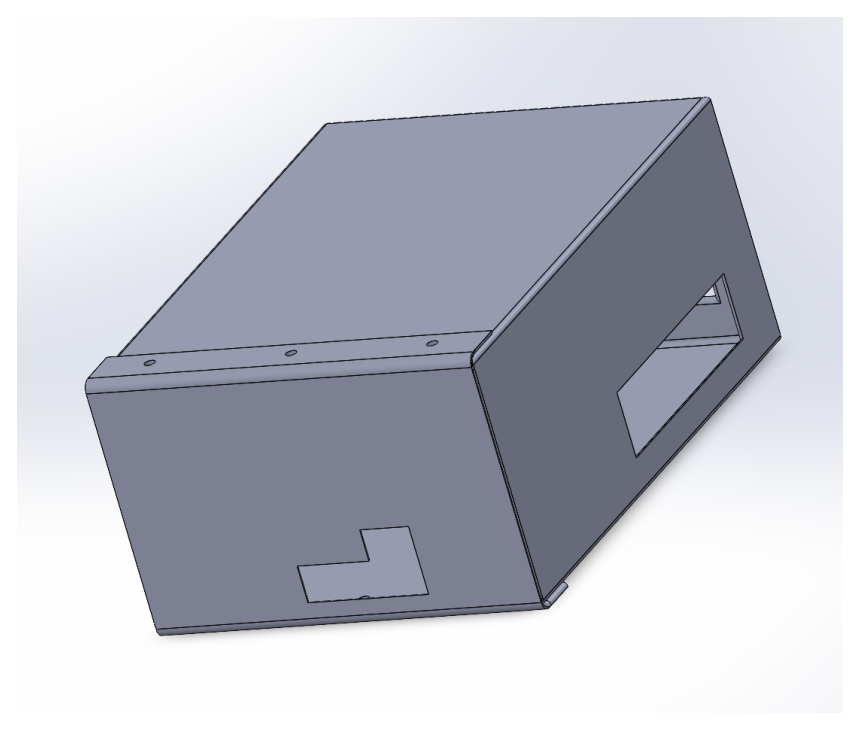
\includegraphics[width=0.40\columnwidth]{fig06a_pi_iso.png}}
\hfil
\subfloat[Camera/gimbal mount]{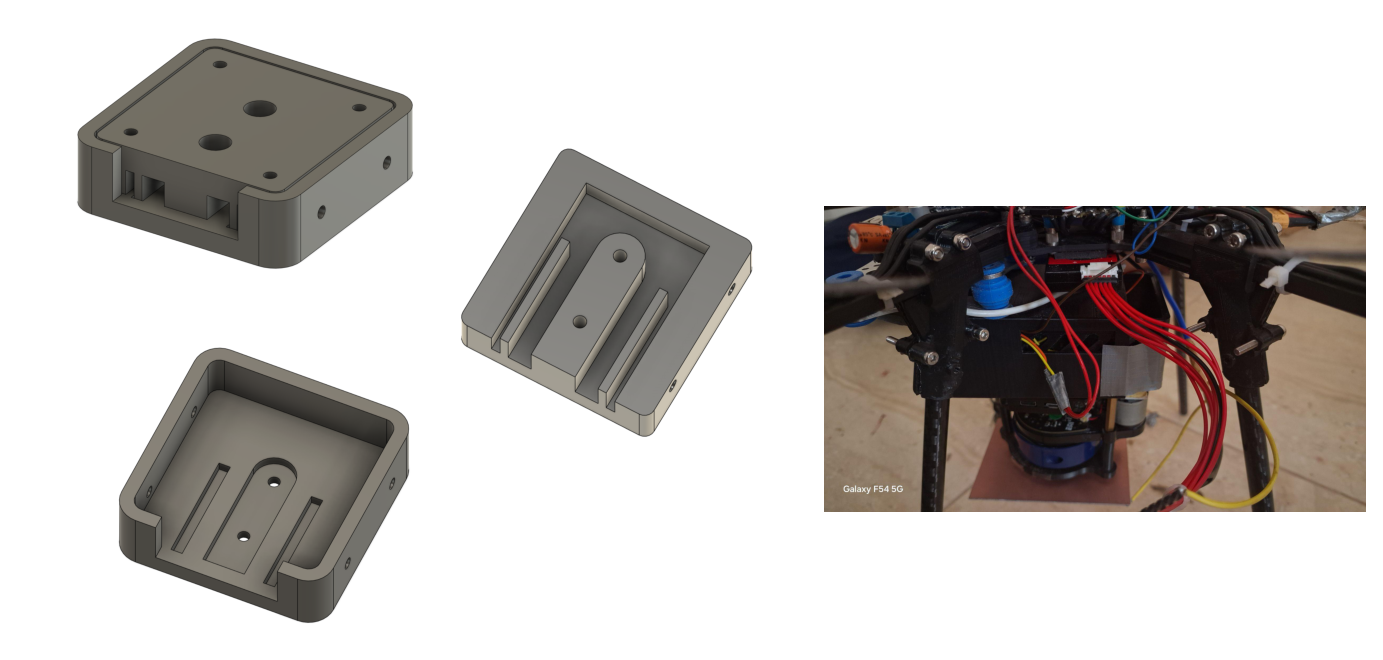
\includegraphics[width=0.50\columnwidth]{fig09_cam.png}}\\
\subfloat[2D LiDAR mount]{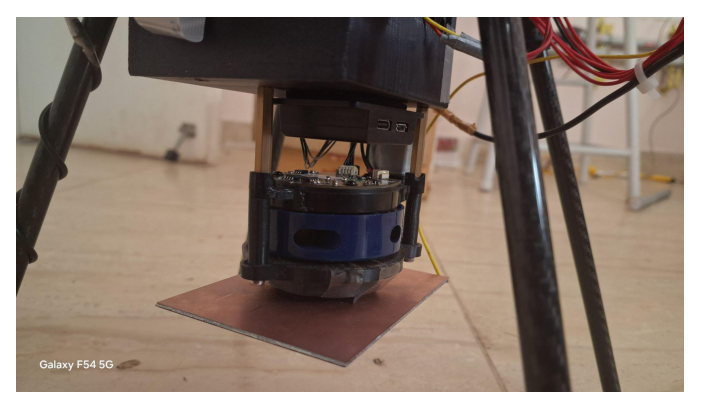
\includegraphics[width=0.40\columnwidth]{fig10_lidar2d.png}}
\hfil
\subfloat[Propeller guards]{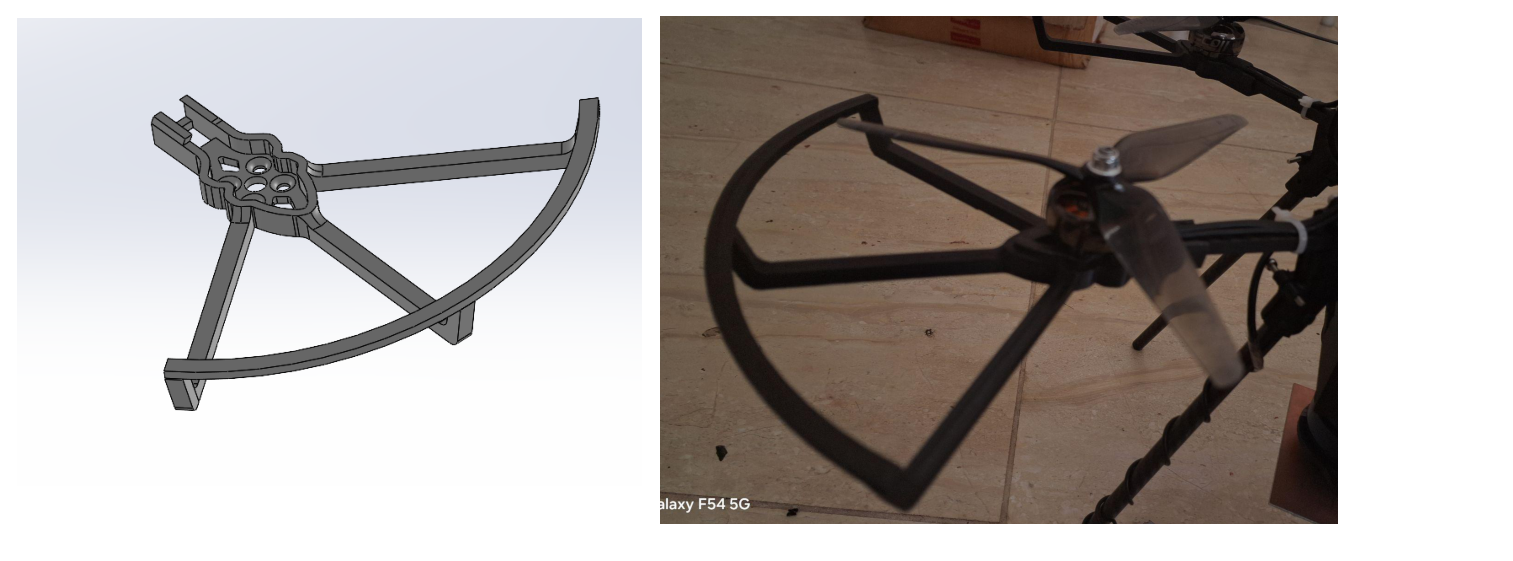
\includegraphics[width=0.50\columnwidth]{fig11_propguard.png}}
\caption{CAD-designed, PLA-printed mounts for the companion computer, camera,
2D LiDAR, and the propeller guards, each iterated for rigidity and low vibration.}
\label{fig:mounts}
\end{figure}

\subsection{Cascaded Flight Control}
A cascaded ArduPilot stack~\cite{ardupilot} organizes flight into three layers
(Fig.~\ref{fig:pid}). The innermost \emph{rate loop} ($400$~Hz--$1$~kHz) maps
desired body rates to motor commands, with gyro sampled to $8$~kHz and filtered
by hardware low-pass and software notch filters. The core law is a PID on the rate
error, \eqref{eq:pid}, augmented by feedforward ($u_{\mathrm{ff}}=r\,K_{\mathrm{ff}}$),
derivative-on-measurement to avoid setpoint kick, and dynamic filter-cutoff
adjustment. The \emph{altitude loop} fuses barometer and downward 1D LiDAR through
a complementary filter/EKF3 with a dynamic hover-throttle estimator. The
\emph{position loop} is driven by onboard optical flow.

\begin{figure}[!t]
\centering
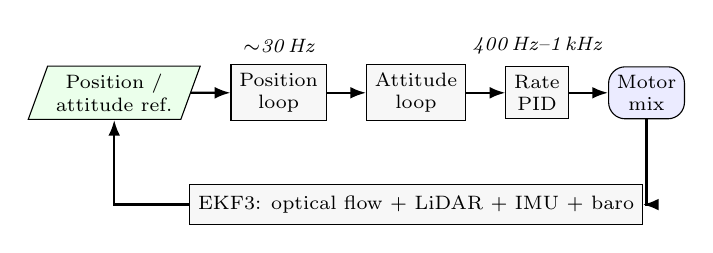
\begin{tikzpicture}[node distance=3mm and 5mm, every node/.style={font=\scriptsize}]
\node[fcio] (ref) {Position /\\attitude ref.};
\node[fcproc, right=of ref] (pos) {Position\\loop};
\node[fcproc, right=of pos] (att) {Attitude\\loop};
\node[fcproc, right=of att] (rate) {Rate\\PID};
\node[fcstart, right=of rate] (mot) {Motor\\mix};
\draw[fcarrow] (ref)--(pos); \draw[fcarrow] (pos)--(att);
\draw[fcarrow] (att)--(rate); \draw[fcarrow] (rate)--(mot);
\node[fcproc, below=8mm of att] (est) {EKF3: optical flow $+$ LiDAR $+$ IMU $+$ baro};
\draw[fcarrow] (mot.south) |- (est.east);
\draw[fcarrow] (est.west) -| (ref.south);
\node[fclabel, above=0.3mm of pos] {$\sim$30\,Hz};
\node[fclabel, above=0.3mm of rate] {400\,Hz--1\,kHz};
\end{tikzpicture}
\caption{Cascaded position--attitude--rate flight-control loop. EKF3 fuses optical
flow, LiDAR, IMU, and barometer to close the GNSS-denied state estimate.}
\label{fig:pid}
\end{figure}

\subsubsection{Optical-Flow Position Hold}
Optical flow is computed on the Raspberry~Pi~5 from the downward global-shutter
camera. Under the brightness-constancy assumption a pixel of intensity $I(x,y,t)$
satisfies
\begin{equation}
I_x u + I_y v + I_t = 0,
\label{eq:bcc}
\end{equation}
where $(u,v)$ is the image-plane velocity and $I_x,I_y,I_t$ are spatial/temporal
gradients. FAST corners~\cite{rosten2006fast} are tracked across frames by
pyramidal Lucas--Kanade~\cite{lucas1981iterative}, normalized, averaged, and sent
to ArduPilot via the MAVLink \texttt{OPTICAL\_FLOW} message. The control cascade is
\begin{align}
e_{\mathrm{pos}} &= p_{\mathrm{target}} - p_{\mathrm{flow}},\\
v_{\mathrm{target}} &= \mathrm{PID}_{\mathrm{pos}}(e_{\mathrm{pos}}),\\
u_{\mathrm{thr}} &= \mathrm{PID}_{\mathrm{vel}}(v_{\mathrm{target}} - v_{\mathrm{flow}}).
\end{align}
EKF3 was reconfigured to treat flow as the primary horizontal source and the
rangefinder as the vertical source (Table~\ref{tab:ekf}), rejecting low-quality
flow under poor texture, motion blur, or altitude uncertainty.

\begin{table}[!t]
\centering
\caption{Key Estimator Parameters for GNSS-Denied Operation}
\label{tab:ekf}
\begin{tabular}{lcl}
\toprule
Parameter & Value & Description\\
\midrule
\texttt{AHRS\_EKF\_TYPE} & 3 & Select EKF3 as active estimator\\
\texttt{EK3\_SRC1\_VELXY} & 5 & Optical flow $\rightarrow$ horiz.\ vel.\\
\texttt{EK3\_SRC1\_POSZ} & 2 & Rangefinder $\rightarrow$ vert.\ position\\
\texttt{EK3\_RNG\_USE\_HGT} & en. & Rangefinder for primary height\\
\bottomrule
\end{tabular}
\end{table}

\subsection{GNSS-Denied Navigation Stack}
Navigation uses a hierarchical two-tier estimator running entirely onboard
(Fig.~\ref{fig:navflow}). \emph{Tier~1} fuses frame-to-frame visual transforms with
IMU in an EKF for a smooth local \texttt{odom}$\rightarrow$\texttt{base\_link} pose;
\emph{Tier~2} is a lower-rate ($5$--$10$~Hz) 2D-LiDAR SLAM
backend~\cite{macenski2021slamtoolbox} that corrects drift by publishing the
\texttt{map}$\rightarrow$\texttt{odom} correction---grounding the vehicle globally
while preserving the smooth local transform the flight controller consumes.
A$^\star$~\cite{hart1968astar} plans over a footprint-inflated 3D costmap;
frontier exploration~\cite{yamauchi1997frontier} drives pilotless coverage; and
6-DOF AMCL~\cite{fox2001amcl} recovers from lost tracking.

\begin{figure}[!t]
\centering
\resizebox{\columnwidth}{!}{%
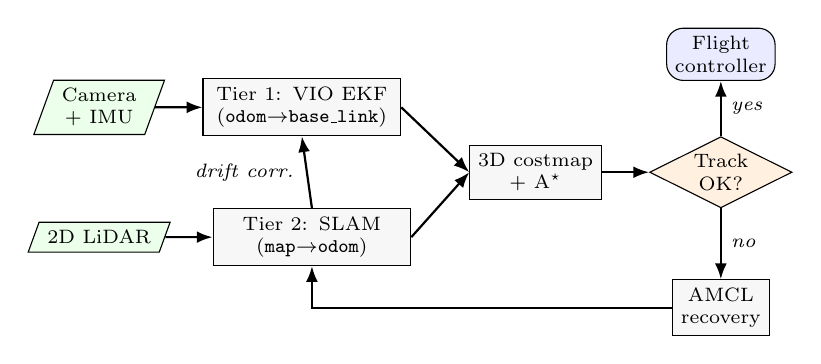
\begin{tikzpicture}[node distance=10mm and 6mm, every node/.style={font=\scriptsize}]
\node[fcio] (cam) {Camera\\$+$ IMU};
\node[fcio, below=11mm of cam] (lid) {2D LiDAR};
\node[fcproc, right=6mm of cam, text width=23mm, align=center] (t1)
  {Tier 1: VIO EKF\\(\texttt{odom}$\to$\texttt{base\_link})};
\node[fcproc, right=6mm of lid, text width=23mm, align=center] (t2)
  {Tier 2: SLAM\\(\texttt{map}$\to$\texttt{odom})};
\coordinate (tmid) at ($(t1.east)!0.5!(t2.east)$);
\node[fcproc, right=8mm of tmid, anchor=west] (cost) {3D costmap\\$+$ A$^\star$};
\node[fcdec, right=6mm of cost] (track) {Track\\OK?};
\node[fcstart, above=7mm of track] (out) {Flight\\controller};
\node[fcproc, below=9mm of track] (amcl) {AMCL\\recovery};
\draw[fcarrow] (cam)--(t1); \draw[fcarrow] (lid)--(t2);
\draw[fcarrow] (t2.north)-- node[fclabel,left=1pt]{drift corr.} (t1.south);
\draw[fcarrow] (t1.east)--(cost.west); \draw[fcarrow] (t2.east)--(cost.west);
\draw[fcarrow] (cost)--(track);
\draw[fcarrow] (track)-- node[fclabel,right]{yes} (out);
\draw[fcarrow] (track)-- node[fclabel,right]{no} (amcl);
\draw[fcarrow] (amcl.west) -| (t2.south);
\end{tikzpicture}}
\caption{GNSS-denied navigation flow: a smooth Tier-1 visual--inertial pose
corrected by a Tier-2 LiDAR-SLAM \texttt{map}$\rightarrow$\texttt{odom} transform,
feeding A$^\star$ planning, with AMCL recovery on tracking loss.}
\label{fig:navflow}
\end{figure}

\subsection{Perception and Validation Pipeline}
Candidate detections are validated against $3$--$5$ seed images through the pipeline
of Fig.~\ref{fig:percflow}. After CLAHE~\cite{pizer1987clahe} normalization,
SIFT~\cite{lowe2004sift} features are matched by FLANN, filtered by Lowe's ratio
test ($d_1<\gamma d_2$, $\gamma\in[0.7,0.75]$) with a mutual cross-check, and
geometrically verified by RANSAC~\cite{fischler1981ransac} fitting a homography
\begin{equation}
[x'\,y'\,1]^\top \sim H\,[x\,y\,1]^\top, \qquad H\in\mathbb{R}^{3\times3}.
\label{eq:homog}
\end{equation}
A detection is declared valid only when inlier count, inlier ratio, and reprojection
error jointly pass strict thresholds.

\begin{figure}[!t]
\centering
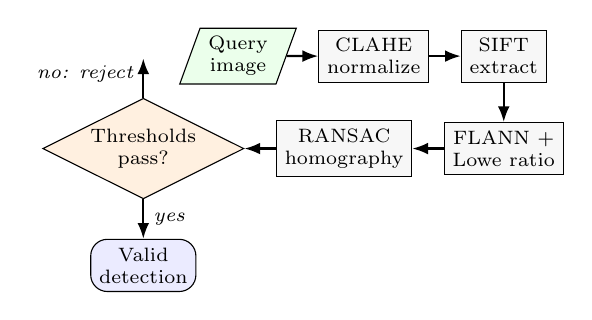
\begin{tikzpicture}[node distance=2.6mm and 4mm, every node/.style={font=\scriptsize}]
\node[fcio] (q) {Query\\image};
\node[fcproc, right=of q] (cl) {CLAHE\\normalize};
\node[fcproc, right=of cl] (sift) {SIFT\\extract};
\node[fcproc, below=5mm of sift] (flann) {FLANN $+$\\Lowe ratio};
\node[fcproc, left=of flann] (ransac) {RANSAC\\homography};
\node[fcdec, left=of ransac] (th) {Thresholds\\pass?};
\node[fcstart, below=5mm of th] (val) {Valid\\detection};
\draw[fcarrow] (q)--(cl); \draw[fcarrow] (cl)--(sift);
\draw[fcarrow] (sift)--(flann); \draw[fcarrow] (flann)--(ransac);
\draw[fcarrow] (ransac)--(th);
\draw[fcarrow] (th)-- node[fclabel,right]{yes} (val);
\draw[fcarrow] (th.north) -- node[fclabel,left,pos=0.6]{no: reject} ++(0,5mm);
\end{tikzpicture}
\caption{Perception validation pipeline: CLAHE normalization, SIFT/FLANN matching
with Lowe's ratio test, and RANSAC homography verification gated by joint inlier
thresholds.}
\label{fig:percflow}
\end{figure}

\subsection{Mission State Machine and Precision Docking}
Execution is organized as a state machine (Fig.~\ref{fig:states}). In the
\emph{Explorer} state the drone maps the unknown environment while detecting and
geo-tagging seed features, flying at a fixed wall offset and emitting dynamic
velocity commands. On meeting objectives or a battery threshold it transitions to
\emph{Return-to-Home}, where Nav2~\cite{macenski2020nav2} computes a collision-free
return over the State~I map. Terminal docking proceeds by (i) HSV masking with
circular hue statistics and CLAHE for outdoor robustness; (ii) shape classification
by circularity/solidity/aspect/extent; and (iii) 2D-LiDAR centering, where a Hough
transform detects the frustum circle and a dedicated PID drives the
center-to-center error to zero for touchdown (Fig.~\ref{fig:centering}).

\begin{figure}[!t]
\centering
\subfloat[Visual centering on the base station]{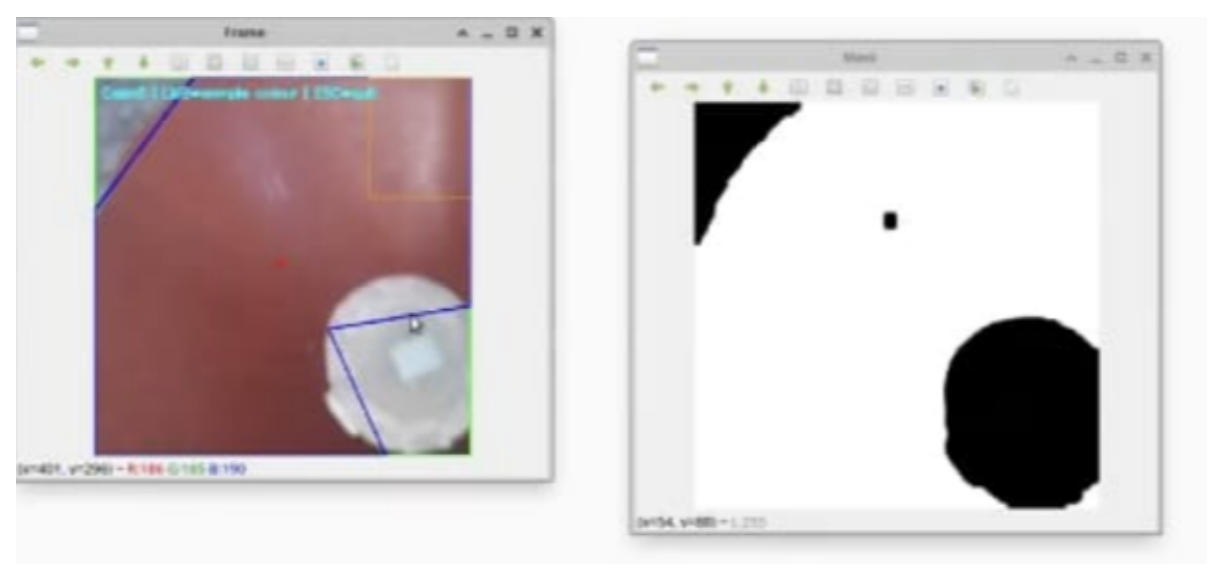
\includegraphics[width=0.50\columnwidth]{fig16_center.png}}
\hfil
\subfloat[2D-LiDAR view during centering]{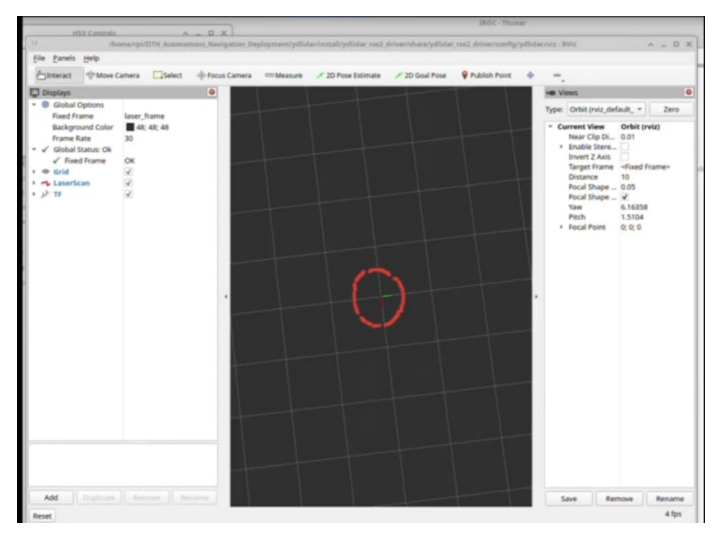
\includegraphics[width=0.40\columnwidth]{fig17_lidarcenter.png}}
\caption{Precision centering combining HSV visual servoing with 2D-LiDAR
Hough-circle detection: as the vehicle enters the frustum the LiDAR traces a
circle whose center error is driven to zero for touchdown.}
\label{fig:centering}
\end{figure}

\begin{figure}[!t]
\centering
\subfloat[Explorer state: mapping and detection.\label{fig:explorer}]
{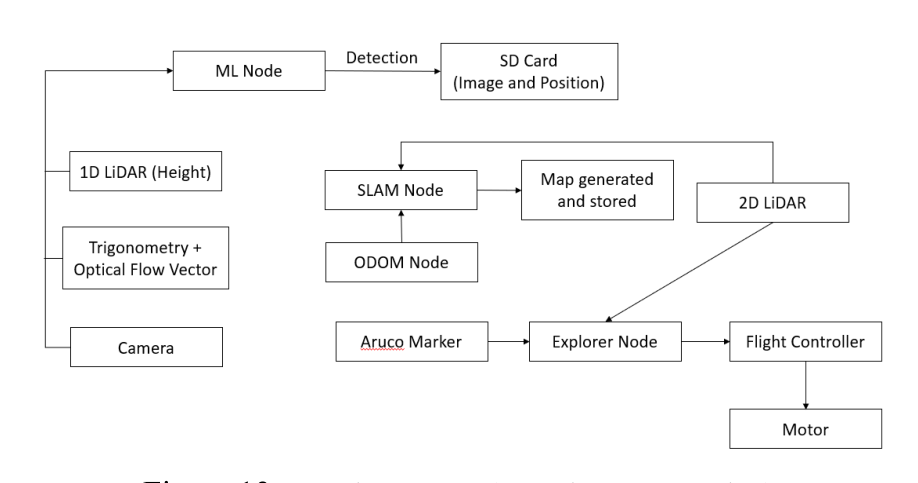
\includegraphics[width=0.49\columnwidth]{drone_explorer.png}}
\hfil
\subfloat[Return-to-home and precision docking.\label{fig:rth}]
{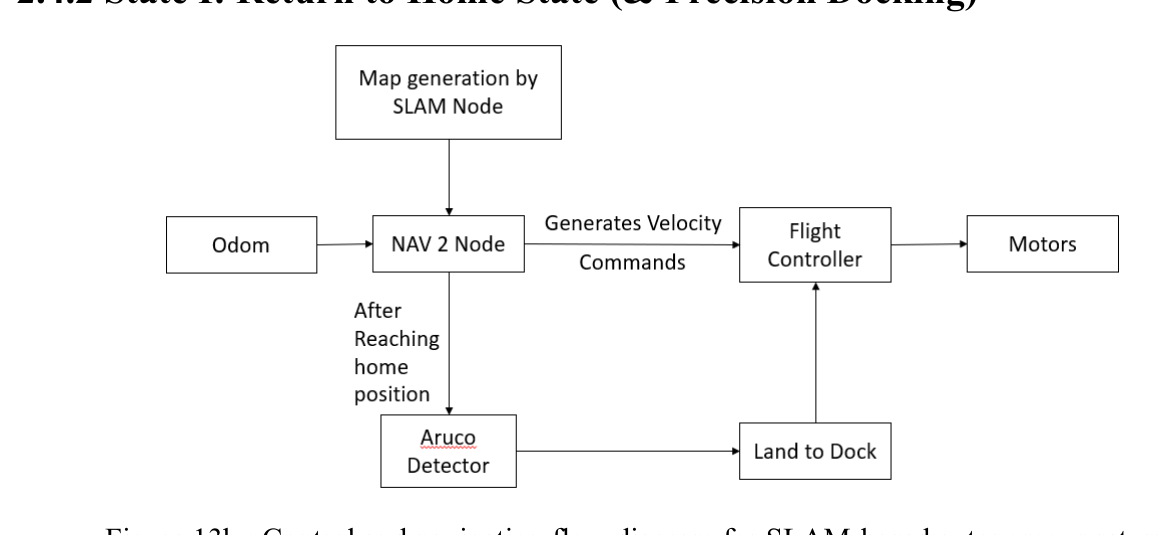
\includegraphics[width=0.49\columnwidth]{drone_rth.png}}
\caption{Mission state machine on the companion computer. State~I prioritizes
coverage and feature logging; State~II prioritizes safe, precise recovery and
docking.}
\label{fig:states}
\end{figure}

\subsection{Hardware, Power Budget, and Safety}
The principal aerial components and their key specifications are listed in
Table~\ref{tab:components}. The power budget is dominated by propulsion: four
motors ($\sim\!400$~W) plus avionics give $\approx\!439$~W, i.e.\ $\sim\!19.8$~A at
$22.2$~V, for a $\sim\!16$-min endurance on a $5600$~mAh pack with a $3.7\times$
discharge-current safety factor (Table~\ref{tab:spec}). Component selection favors
endurance and integration robustness: low-KV motors with low-pitch propellers give
a low hover throttle, and the architecture is companion-computer-centric, so the
F4-class controller handles only high-rate stabilization while the Pi/Jetson runs
autonomy. Safety is layered: a hardware kill switch cuts motor power in
$<\!200$~ms, a MAVLink manual override (FlySky AFHDS~2A) hands authority to a pilot,
and automatic failsafes cover battery, radio, and EKF position-estimate failure.

\begin{table}[!t]
\centering
\caption{Principal Aerial Hardware and Key Specifications}
\label{tab:components}
\begin{tabular}{p{1.7cm}p{2.4cm}p{2.6cm}}
\toprule
Subsystem & Component & Key specification\\
\midrule
Airframe      & GEPRC Mark4 8\,in     & Carbon fiber, $450$\,mm\\
Propulsion    & Emax 2807 $1300$\,KV $\times4$ & $7030$ props, $\sim\!400$\,W\\
ESC           & Hobbywing 4-in-1      & $\sim\!1.5\times$ peak headroom\\
Flight ctrl.  & SpeedyBee F4 / Pixhawk & Rate/attitude, $8$\,kHz gyro\\
Companion     & Raspberry~Pi~5        & Optical flow, SLAM, perception\\
GPU (planned) & Jetson Orin~Nano      & CUDA/TensorRT CNN inference\\
Flow camera   & Arducam OV9281        & Global shutter, MIPI-CSI\\
1D LiDAR      & Benewake TFmini-S     & $0.1$--$12$\,m, $1$\,kHz alt.\\
2D LiDAR      & YDLIDAR~X2            & $360^\circ$ SLAM / docking\\
Battery       & 6S LiPo $5600$\,mAh   & $22.2$\,V, BMS-protected\\
\bottomrule
\end{tabular}
\end{table}

\begin{table}[!t]
\centering
\caption{Aerial System Specification}
\label{tab:spec}
\begin{tabular}{ll}
\toprule
Parameter & Specification\\
\midrule
Overall mass        & $1900$\,g\\
Overall dimensions  & $450\times500\times350$\,mm\\
Power requirement   & $300$--$500$\,W\\
Flight time/charge  & $10$--$15$\,min\\
Propellers          & $4\times7030$\\
Key features        & GNSS-denied nav., image recognition, auto-docking\\
\bottomrule
\end{tabular}
\end{table}

\subsection{End-to-End Development and Bring-Up}
The aerial platform was developed as a staged, end-to-end bring-up so that each
capability was validated before the next was layered on. (1)~\emph{Airframe and
propulsion.} The carbon frame was assembled, motors and the 4-in-1 ESC mounted,
and thrust/throttle characterized to confirm the hover-throttle and endurance
budget of Table~\ref{tab:spec}. (2)~\emph{Manual flight and tuning.} ArduCopter
was flashed and the cascaded rate/attitude loops tuned from blackbox logs, with
the software notch filters set to the measured vibration harmonics.
(3)~\emph{Sensor calibration.} The IMU, external magnetometer, barometer, and the
1D/2D LiDARs were calibrated and time-synchronized to the EKF3.
(4)~\emph{GNSS-denied position hold.} The optical-flow pipeline was brought up on
the Pi, EKF3 re-sourced to flow and rangefinder (Table~\ref{tab:ekf}), and
centimeter-level hover verified. (5)~\emph{Autonomy.} The two-tier estimator and
2D-LiDAR SLAM were enabled, frontier exploration and the perception pipeline
integrated as ROS2 nodes, and the Explorer/Return-to-Home state machine exercised.
(6)~\emph{Docking and charging.} The frustum descent, HSV/Hough centering, and
magnetic auto-charging were tuned last, closing the persistence loop. This staged
workflow---airframe, flight, sensing, position hold, autonomy, recovery---kept
faults isolated to a single newly added layer and mirrors the order in which the
subsystems are presented above.

\section{Hierarchical Path Planning and Swarm Coordination}
\label{sec:planning}

\subsection{Dynamic Models for Planning}
The aquatic agent is modeled as a planar 3-DOF body with state
$p=[x,\,y,\,\psi]^\top$ subject to surge $u$, sway $v$, yaw rate $r$, and current
$(v_{cx},v_{cy})$:
\begin{align}
\dot{x} &= u\cos\psi - v\sin\psi + v_{cx},\\
\dot{y} &= u\sin\psi + v\cos\psi + v_{cy},\qquad \dot{\psi} = r,
\end{align}
with thrust $F_t$ and yaw torque $\tau_z$ supplied through the CPG and the
CFD-derived hydrodynamic forces. The aerial agent is a 6-DOF quadrotor governed
by Newton--Euler dynamics, $\ddot{p} = \tfrac{1}{m}R\,T - g + d$, with rotation
matrix $R$, mass $m$, total thrust $T$, gravity $g$, and disturbance $d$,
stabilized by the Pixhawk.

\subsection{Two-Level PSO--MPC Planner}
Planning is hierarchical. A \emph{global} PSO layer~\cite{kennedy1995particle}
encodes each candidate path as a waypoint sequence and evolves a particle
population by
\begin{equation}
v_i^{k+1} = w\,v_i^{k} + c_1 r_1(\mathrm{pbest}_i - x_i^{k})
          + c_2 r_2(\mathrm{gbest} - x_i^{k}),
\end{equation}
$x_i^{k+1}=x_i^{k}+v_i^{k+1}$, minimizing a multi-objective fitness
\begin{equation}
J = w_1 J_{\mathrm{length}} + w_2 J_{\mathrm{energy}}
  + w_3 J_{\mathrm{smooth}} + w_4 J_{\mathrm{collision}},
\label{eq:psocost}
\end{equation}
that trades path length, propulsion energy, smoothness, and obstacle clearance.
A \emph{local} MPC layer~\cite{mayne2000constrained,yan2022bionic} then tracks the
global reference over a horizon $H_p$ under disturbances,
\begin{equation}
J_{\mathrm{MPC}} = \sum_{k=0}^{H_p}
\Big(\lVert p_{\mathrm{ref}}(k) - p(k)\rVert_Q^2 + \lVert u_c(k)\rVert_R^2\Big),
\label{eq:mpc}
\end{equation}
subject to the agent dynamics and input/state bounds. For the fish, the MPC output
modulates the CPG amplitude and frequency in \eqref{eq:cpg}, closing the loop from
mission planning to rhythmic actuation; for the drone, it issues velocity commands
to the cascaded flight stack. ADAPTH supplies cross-domain updates (current shifts,
target detections) that trigger global re-planning. In simulation the framework
reduced global path length by $\sim\!25\%$ relative to an A$^\star$ baseline and
achieved $90\%$ tracking accuracy with RMSE below $0.1$~m under disturbance.

\subsection{Controlled Graph-Theoretic Formation Study}
To characterize swarm-level behavior under a bio-inspired motion regime, we ran a
controlled study on a state-of-the-art graph-theoretic formation
planner~\cite{quan2022distributed} in which seven agents hold a hexagonal template
through a cluttered random forest. The planner represents the swarm as a complete
weighted graph with normalized Laplacian $\hat{L}$ and penalizes a
formation-similarity cost
$f_{\mathrm{form}}=\lVert \hat{L}-\hat{L}^{\mathrm{des}}\rVert_F^2$, jointly
optimized with obstacle, smoothness, and dynamic-feasibility terms over a
MINCO~\cite{wang2022geometrically} trajectory. Holding planner, cost weights,
template, and obstacle field fixed, we contracted only the
\emph{dynamic-feasibility envelope} from quadrotor values to fish-like values
($v_{\max}\!:\!1.5\!\rightarrow\!1.0$~m/s,
$a_{\max}\!:\!8.0\!\rightarrow\!2.5$~m/s$^2$) and recorded a paired, headless
experiment at $100$~Hz over five obstacle seeds per condition (the same seed yields
the same forest in both conditions). The fish-like envelope roughly \emph{halves}
RMS jerk and cuts mean acceleration by $\sim\!44\%$---visibly smoother,
drag-limited motion---at the cost of $\sim\!44\%$ longer traversal, while formation
accuracy, inter-agent spacing, obstacle clearance, and a $100\%$ success rate are
preserved within run-to-run noise (Table~\ref{tab:formresults},
Figs.~\ref{fig:swarm_traj}--\ref{fig:swarm_rviz}). This shows that a
high-performance formation planner degrades gracefully under the slow, smooth
regime the hydrodynamic analysis recommends, and that the graph-similarity cost is
largely decoupled from the aggressiveness of the underlying motion---a useful
robustness property for slow, drag-limited platforms.

\begin{table*}[t]
\caption{Controlled Formation Study: Aggregate Results Across Five Obstacle Seeds
Per Condition (Mean~$\pm$~Std). Only the Dynamic Envelope Differs Between Columns.}
\label{tab:formresults}
\centering
\begin{tabular}{llcccc}
\toprule
\textbf{Metric} & \textbf{Unit} & \textbf{Baseline (quadrotor)} &
\textbf{Fish-like envelope} & \textbf{Change} & \textbf{Category}\\
\midrule
Max speed              & m/s     & $1.581 \pm 0.014$ & $1.126 \pm 0.047$ & $-29\%$ & Kinematic\\
Mean speed             & m/s     & $0.976 \pm 0.030$ & $0.726 \pm 0.068$ & $-26\%$ & Kinematic\\
Max accel              & m/s$^2$ & $1.355 \pm 0.249$ & $0.854 \pm 0.383$ & $-37\%$ & Kinematic\\
Mean accel             & m/s$^2$ & $0.218 \pm 0.025$ & $0.123 \pm 0.031$ & $-44\%$ & Kinematic\\
\textbf{RMS jerk}      & m/s$^3$ & $0.658 \pm 0.116$ & $\mathbf{0.338 \pm 0.129}$ & $\mathbf{-49\%}$ & Kinematic\\
Path length            & m       & $51.420 \pm 0.224$ & $52.325 \pm 0.372$ & $+1.8\%$ & Efficiency\\
\textbf{Traversal time}& s       & $44.919 \pm 1.433$ & $\mathbf{64.501 \pm 4.327}$ & $\mathbf{+44\%}$ & Efficiency\\
Formation RMSE (mean)  & m       & $0.176 \pm 0.023$ & $0.217 \pm 0.026$ & $+24\%$ & Formation\\
Formation RMSE (max)   & m       & $0.774 \pm 0.078$ & $0.799 \pm 0.208$ & $+3\%$ & Formation\\
Min inter-agent dist   & m       & $1.599 \pm 0.354$ & $1.705 \pm 0.453$ & $+7\%$ & Safety\\
Mean obstacle clearance& m       & $1.116 \pm 0.068$ & $1.094 \pm 0.077$ & $-2\%$ & Safety\\
Near-miss frac.\ ($<0.3$~m) & --  & $0.058 \pm 0.014$ & $0.066 \pm 0.013$ & $+14\%$ & Safety\\
Success rate           & \%      & $100$ & $100$ & $0$ & Safety\\
\bottomrule
\end{tabular}
\end{table*}

\begin{figure*}[t]
\centering
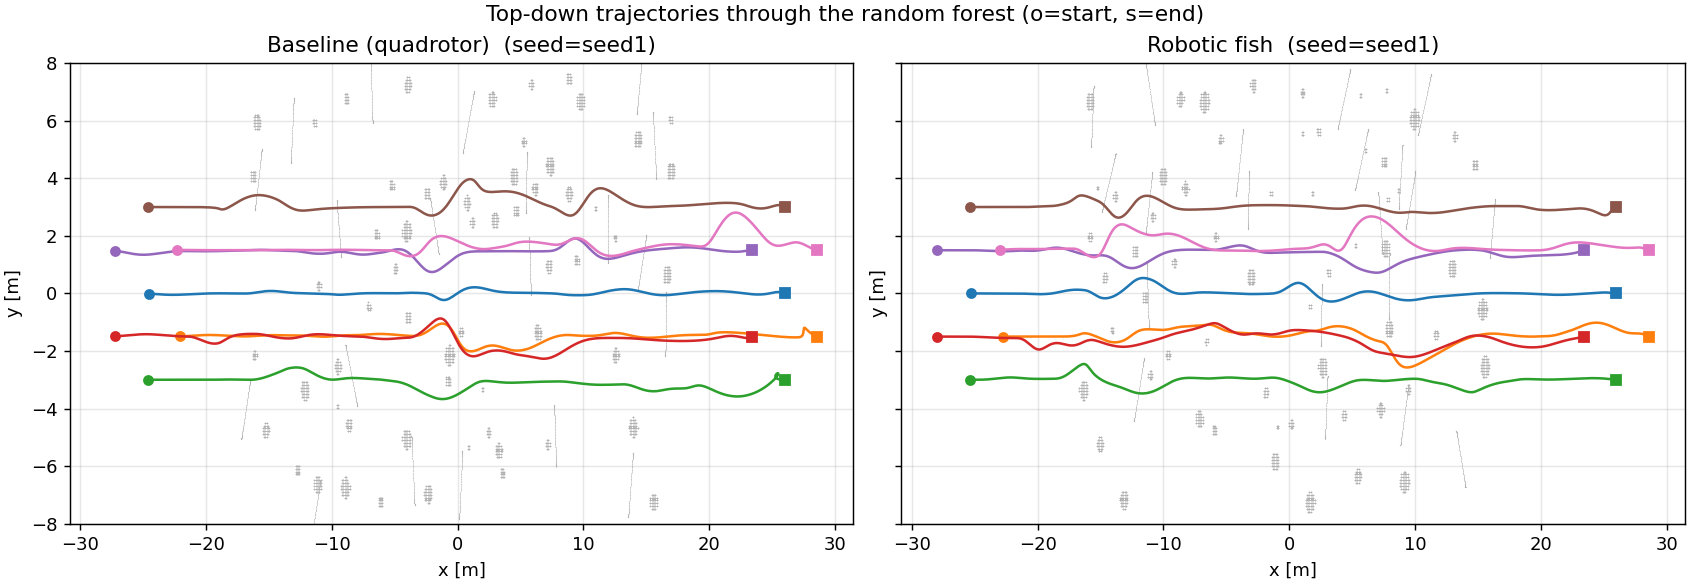
\includegraphics[width=0.86\textwidth]{swarm_trajectories.png}
\caption{Top-down executed paths through the random forest (seed~1), baseline
(left) versus fish-like envelope (right). $\bigcirc$ marks the start hexagon,
$\square$ the goal; path length differs by under $2\%$.}
\label{fig:swarm_traj}
\end{figure*}

\begin{figure*}[t]
\centering
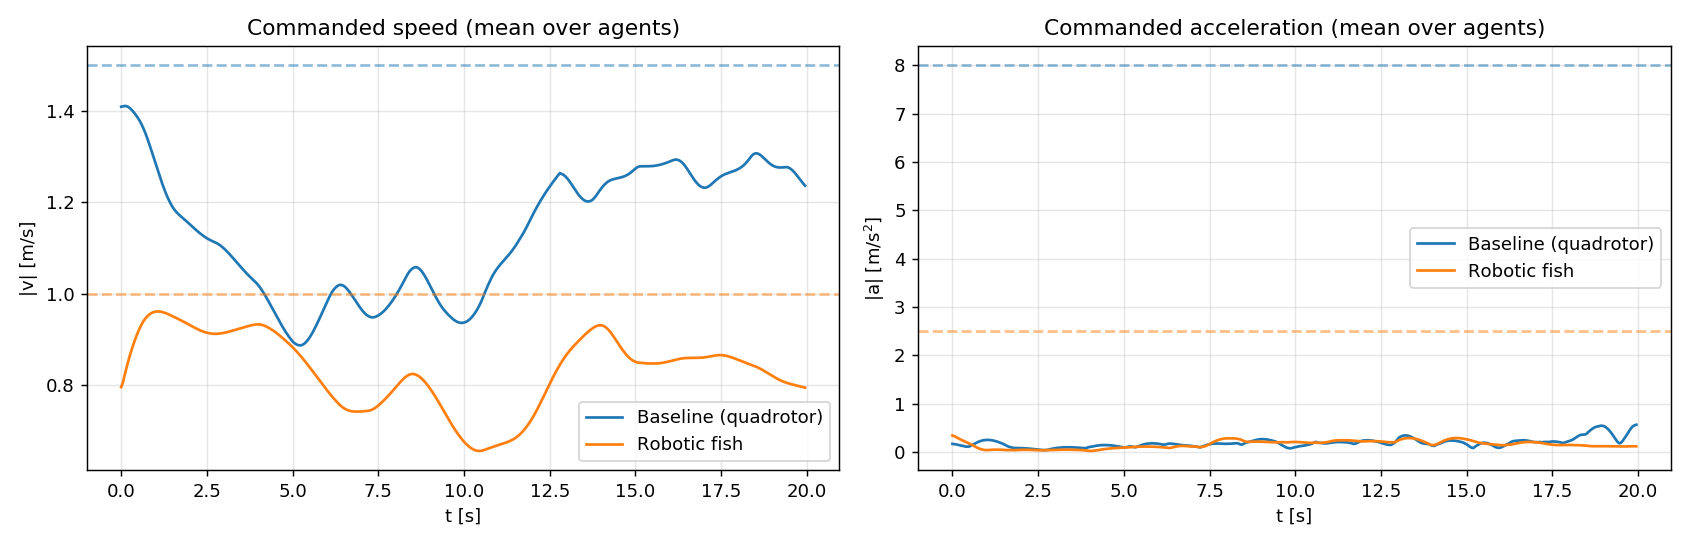
\includegraphics[width=0.86\textwidth]{swarm_kinematics.png}
\caption{Commanded speed (top) and acceleration (bottom), averaged over the
seven agents, for the first $20$~s. Dashed lines are the per-condition $v_{\max}$
and $a_{\max}$. The fish-like envelope yields lower, flatter, smoother profiles.}
\label{fig:swarm_kin}
\end{figure*}

\begin{figure*}[t]
\centering
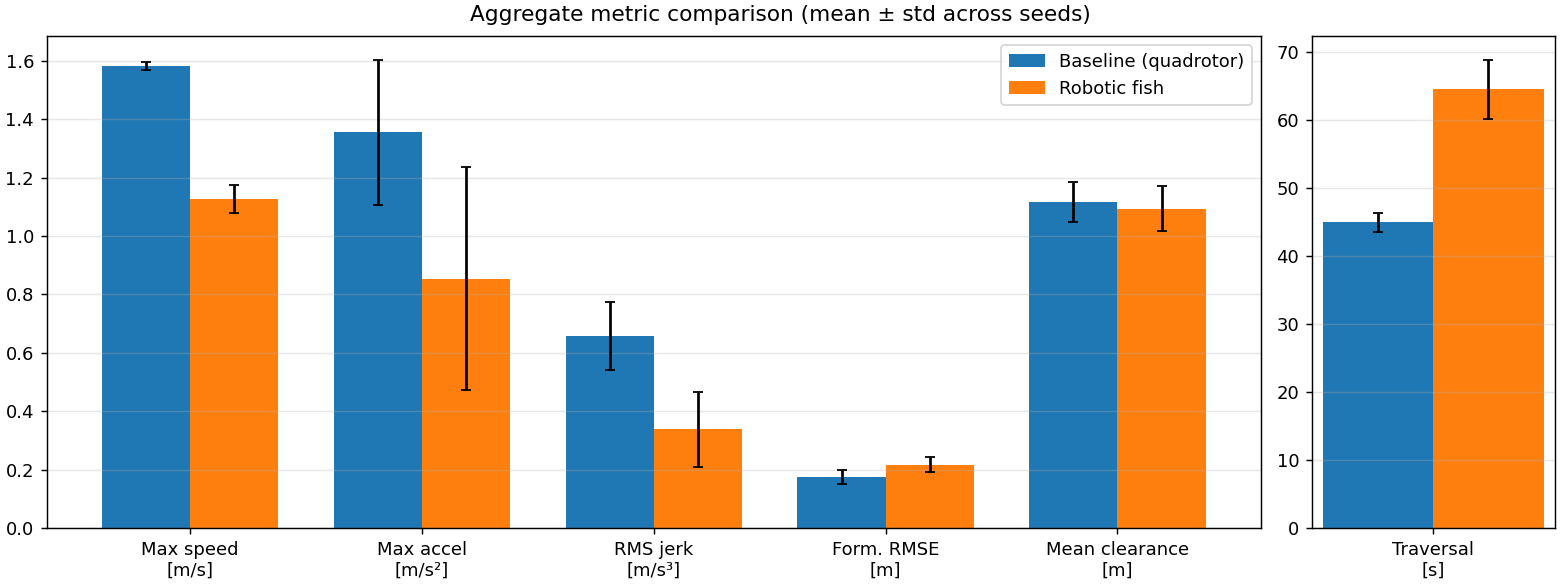
\includegraphics[width=0.86\textwidth]{swarm_bars.png}
\caption{Aggregate comparison (mean~$\pm$~std over five seeds). Kinematic
smoothness improves substantially and traversal time grows, while formation
accuracy, clearance, and safety remain within noise.}
\label{fig:swarm_bars}
\end{figure*}

\begin{figure}[t]
\centering
\subfloat[Mid-field hexagon school.]{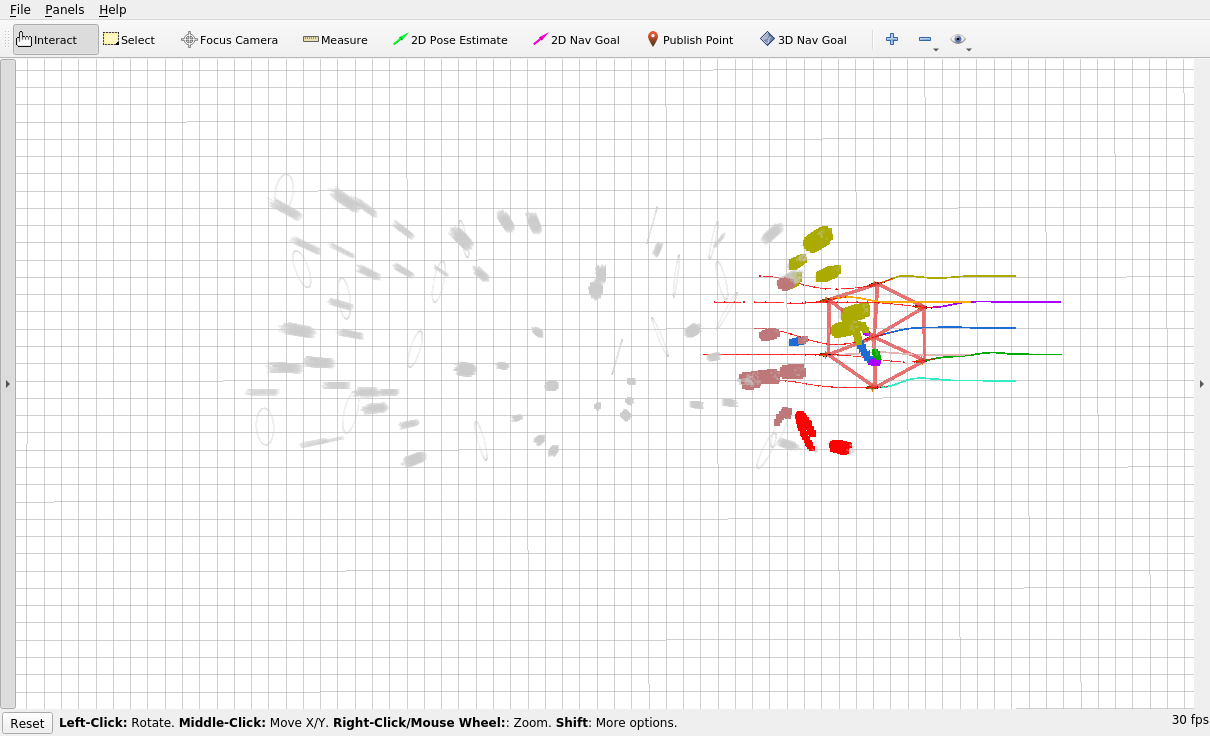
\includegraphics[width=0.49\columnwidth]{swarm_rviz_midfield.png}}
\hfil
\subfloat[All seven executed paths.]{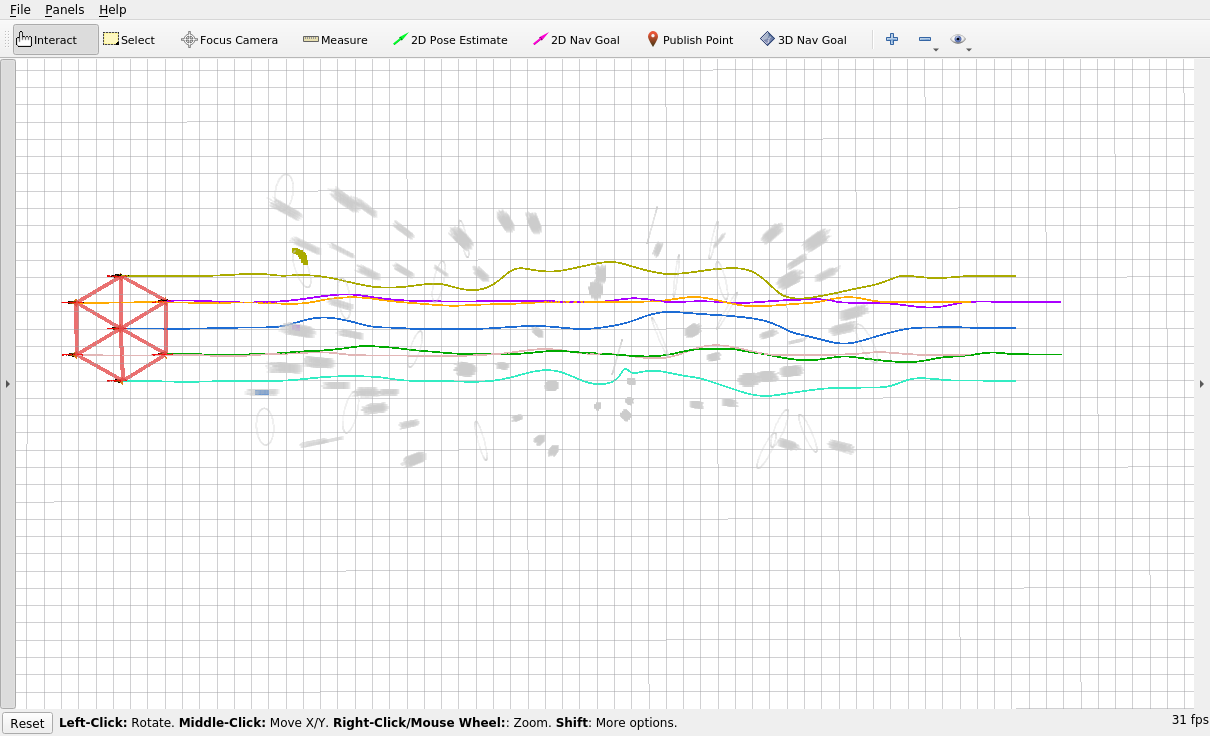
\includegraphics[width=0.49\columnwidth]{swarm_rviz_paths.png}}
\caption{Qualitative RViz views (fish-like condition, seed~1): the seven-agent
hexagon school weaving through the obstacle forest, and the full set of executed
trajectories from start to goal.}
\label{fig:swarm_rviz}
\end{figure}

\subsection{Graph-Theoretic Formation Formulation}
The substrate planner represents the instantaneous swarm as a complete weighted
graph whose $N$ vertices are the agent positions $p_i\in\mathbb{R}^3$, with edge
weights $A_{ij}=\lVert p_i-p_j\rVert_2^2$, degree $d_i=\sum_j A_{ij}$, and
symmetric normalized Laplacian
\begin{equation}
\hat{L}_{ij}=
\begin{cases}
1, & i=j,\\[2pt]
-A_{ij}\,d_i^{-1/2}\,d_j^{-1/2}, & i\neq j .
\end{cases}
\end{equation}
Given a desired template with Laplacian $\hat{L}^{\mathrm{des}}$, the
formation-similarity cost is the squared Frobenius norm of the Laplacian
difference,
\begin{equation}
f_{\mathrm{form}}=\big\lVert\hat{L}-\hat{L}^{\mathrm{des}}\big\rVert_F^2 ,
\label{eq:fform}
\end{equation}
which is invariant to translation, rotation, and uniform scaling of the formation
and is differentiable in the positions, so its analytic gradient propagates to
each agent's trajectory. Each agent optimizes a
MINCO~\cite{wang2022geometrically} polynomial against a joint cost
\begin{equation}
J_{\mathrm{swarm}} = \lambda_f f_{\mathrm{form}} + \lambda_o f_{\mathrm{obs}}
  + \lambda_s f_{\mathrm{smooth}} + \lambda_d f_{\mathrm{dyn}},
\label{eq:Jswarm}
\end{equation}
where $f_{\mathrm{obs}}$ penalizes obstacle and inter-agent collision,
$f_{\mathrm{smooth}}$ is minimum-jerk control effort, and $f_{\mathrm{dyn}}$
penalizes violation of the dynamic-feasibility envelope $\{v_{\max},a_{\max}\}$.
The optimization is \emph{decentralized}: each agent solves its own problem using
broadcast neighbor trajectories, so the scheme scales with team size and has no
single point of failure---a property essential for a field-deployed school. The
hexagon template (one centroid, six vertices) was chosen because it packs the
seven agents at the close, near-uniform spacing the CFD analysis identifies as
energetically favorable while leaving each agent a clear obstacle-avoidance
corridor.

\subsection{Fish-School Realization}
Rendering each agent as a robotic fish and contracting the envelope yields the
school behavior of Fig.~\ref{fig:fishswarm}: seven fish hold the hexagon while
weaving through the forest, gliding rather than darting in line with the halved
jerk. The executed trajectories remain smooth and nearly equal in length to the
quadrotor baseline, confirming that the bio-inspired embodiment and the slow,
drag-limited envelope are compatible with the graph-theoretic planner without any
change to its optimization core.

\begin{figure}[t]
\centering
\subfloat[Executed fish-school trajectories]{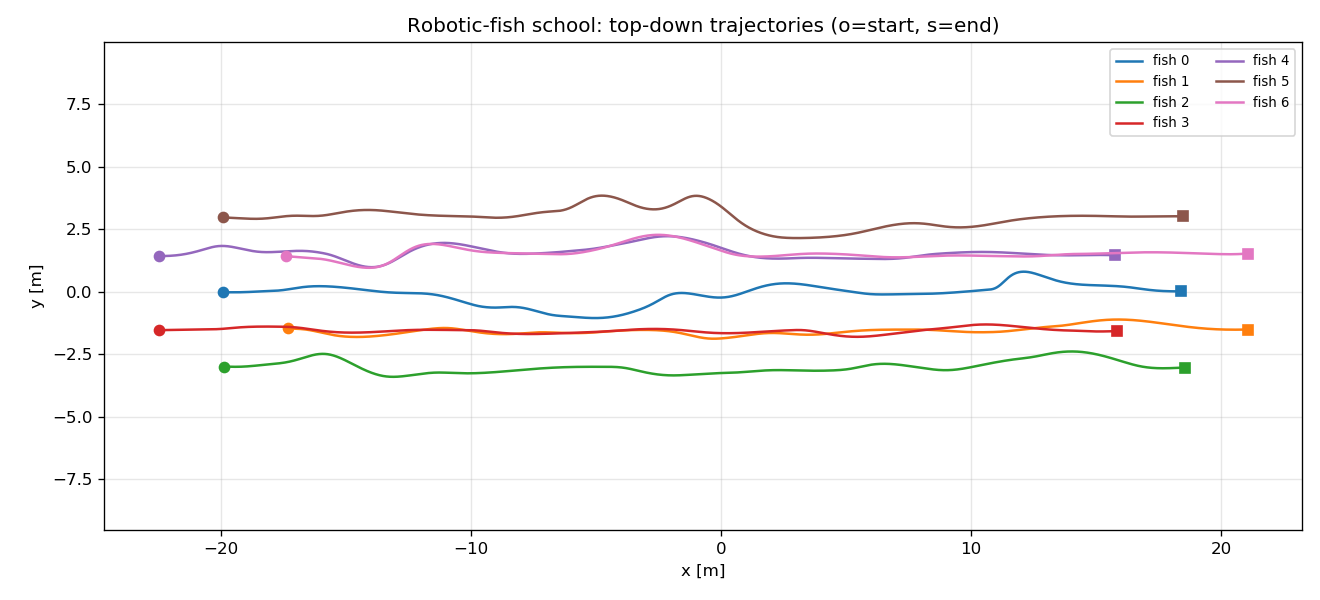
\includegraphics[width=0.49\columnwidth]{fish_swarm_traj.png}}
\hfil
\subfloat[RViz fish-school capture]{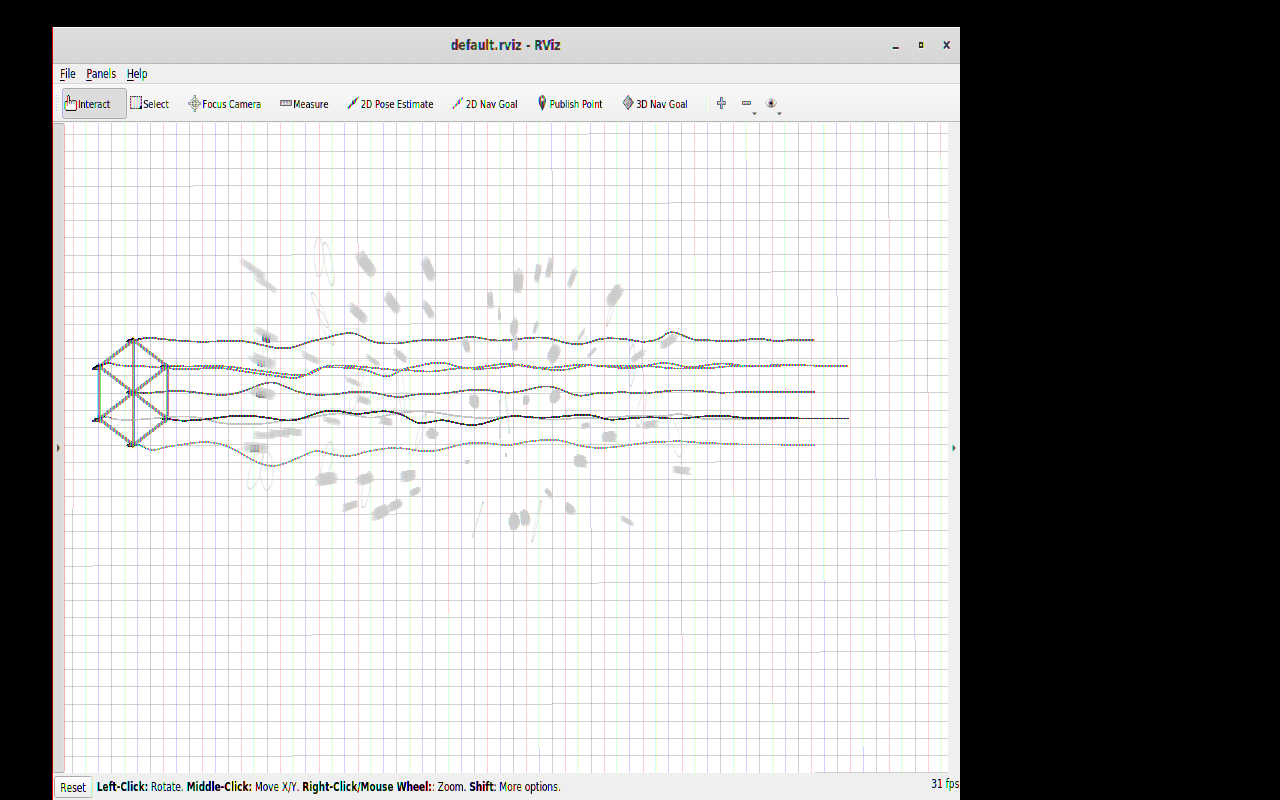
\includegraphics[width=0.49\columnwidth]{fish_swarm_rviz.png}}
\caption{Robotic-fish swarm realization of the graph-theoretic formation planner:
executed trajectories of the seven-agent school and an RViz capture of the
fish-rendered hexagon traversing the obstacle field.}
\label{fig:fishswarm}
\end{figure}

\section{ADAPTH: Adaptive Cross-Domain Communication Protocol}
\label{sec:adapth}
The principal novelty of this work is \emph{ADAPTH} (Adaptive Dynamic
Aerial--Aquatic Path-Tracking and Hybridization), a communication protocol that
bridges the electromagnetically incompatible air and water channels and sustains
coordinated swarm behavior across them.

\subsection{Problem and Design Principles}
Air and water impose asymmetric links: aerial RF achieves millisecond latency and
high bandwidth, while underwater acoustic links incur delays up to $2$~s with low
bandwidth (Table~\ref{tab:comm}). Generic MAC schemes such as TDMA or CSMA/CA are
ill-suited to this asymmetry. ADAPTH is built on three principles:
(i) \emph{medium translation} through a surface relay that terminates an RF/Wi-Fi
link on the air side and an acoustic/ESP-NOW link on the water side;
(ii) \emph{mission prioritization}, so that time-critical events (target
detections, current-shift alerts) preempt routine telemetry; and
(iii) a \emph{wait-and-verify handshake} with packet-wrapping and error correction
that tolerates the long, variable acoustic delay without stalling the aerial
control loop.

\subsection{Architecture}
ADAPTH comprises three node types (Fig.~\ref{fig:adapth_arch}):
\begin{itemize}
  \item \textbf{Aerial node (Raspberry~Pi~5).} Runs perception (camera via
  OpenCV), decision-making (the PSO--MPC predictor), and ADAPTH packetization,
  interfacing with the Pixhawk over MAVLink/UART.
  \item \textbf{Aquatic node (ESP32).} Runs navigation (IMU/magnetometer fusion),
  propulsion (CPG tail oscillation), and execution (PWM to the DC motor),
  communicating over ESP-NOW/Wi-Fi.
  \item \textbf{Wireless gateway (laptop/buoy).} Routes packets, translates
  semantics across domains (e.g., a drone ``Search'' command into a fish ``CPG
  bias''), and maintains the dual sockets for the RF--Wi-Fi and acoustic legs.
\end{itemize}
The relay co-locates with the charging base station, so a docked drone doubles as
a high-bandwidth uplink while it recharges, and asynchronous synchronization
handles the $0.5$--$2$~s latency band.

\begin{figure}[!t]
\centering
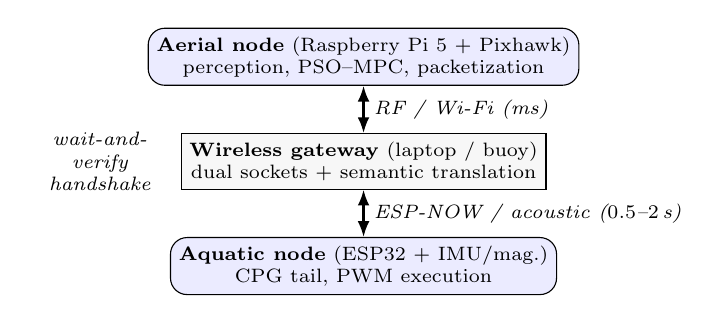
\begin{tikzpicture}[node distance=6mm, every node/.style={font=\scriptsize}]
\node[fcstart] (air) {\textbf{Aerial node} (Raspberry~Pi~5 $+$ Pixhawk)\\
  perception, PSO--MPC, packetization};
\node[fcproc, below=of air] (gw) {\textbf{Wireless gateway} (laptop / buoy)\\
  dual sockets $+$ semantic translation};
\node[fcstart, below=of gw] (aq) {\textbf{Aquatic node} (ESP32 $+$ IMU/mag.)\\
  CPG tail, PWM execution};
\draw[{Latex[length=2mm]}-{Latex[length=2mm]}, thick] (air) --
  node[fclabel, right] {RF / Wi-Fi (ms)} (gw);
\draw[{Latex[length=2mm]}-{Latex[length=2mm]}, thick] (gw) --
  node[fclabel, right] {ESP-NOW / acoustic ($0.5$--$2$\,s)} (aq);
\node[fclabel, left=1mm of gw, align=center, text width=1.6cm]
  {wait-and-verify handshake};
\end{tikzpicture}
\caption{ADAPTH architecture flow: a surface gateway bridges the low-latency aerial
RF domain and the high-latency aquatic acoustic domain, translating semantics and
maintaining bidirectional, wait-and-verify feedback.}
\label{fig:adapth_arch}
\end{figure}

\subsection{Protocol Workflow}
ADAPTH supports bidirectional, feedback-driven coordination:
\begin{enumerate}
  \item A fish detects an environmental change (e.g., a current shift via its
  magnetometer) and sends an alert to the gateway.
  \item The gateway forwards the alert to the drone, which updates its PSO--MPC
  plan and adjusts position to maintain the cross-domain formation.
  \item Conversely, the drone detects a target via its camera and sends a GPS
  offset to the gateway, which translates it into a CPG bias that steers the fish
  toward the target.
\end{enumerate}
Each exchange uses the wait-and-verify handshake: the sender wraps the payload
with a sequence number and checksum, the receiver acknowledges only on successful
verification, and unacknowledged mission-critical packets are retransmitted under
a priority schedule while routine telemetry degrades gracefully. Link quality is
tracked online as a success-rate metric, targeting $85\%$ delivery in noisy
conditions. Lightweight on-node models keep decisions local; for example, the fish
CPG of \eqref{eq:cpg} is biased directly by translated gateway commands.

\subsection{Implementation}
ADAPTH is implemented as a thin, layered stack on top of commodity radios so that
no custom physical layer is required. \emph{Physical/link layer:} the aerial leg
uses Wi-Fi/RF between the Pi~5 and the gateway, while the aquatic leg uses ESP-NOW
(a connectionless, low-overhead $2.4$~GHz protocol) at the surface and an acoustic
modem sub-surface; the gateway terminates both. \emph{Packet layer:} every ADAPTH
frame carries a fixed header---source/destination identifiers, a message-type code
(e.g.\ \texttt{ALERT}, \texttt{TARGET}, \texttt{CMD}, \texttt{TELEMETRY}), a
priority flag, a monotonic sequence number, and a checksum---followed by a compact
payload (a GPS offset, a current-shift vector, or a CPG bias triple
$\{A,\omega,\phi\}$). Keeping payloads small is essential on the bandwidth-limited
acoustic leg. \emph{Routing/translation layer:} the gateway maintains two sockets,
one per medium, and a translation table that maps domain-specific semantics across
the boundary---for instance a drone \texttt{TARGET} (GPS offset) is rewritten as a
fish \texttt{CMD} that biases the CPG of \eqref{eq:cpg} toward the target heading.

\emph{Handshake and reliability:} the wait-and-verify exchange is a small state
machine. The sender transmits a framed packet and starts a timer scaled to the
medium's expected latency (milliseconds for RF, up to seconds for acoustic). The
receiver verifies the checksum and replies with an \texttt{ACK} carrying the echoed
sequence number; on timeout the sender retransmits, but \emph{only} high-priority
\texttt{ALERT}/\texttt{TARGET}/\texttt{CMD} frames are retried aggressively, while
\texttt{TELEMETRY} is allowed to drop so the link never saturates on stale data.
Because the aerial control loop must not block on the slow acoustic leg, exchanges
are \emph{asynchronous}: the Pi~5 continues planning and flying while outstanding
aquatic acknowledgements are pending, reconciling state when the \texttt{ACK}
finally arrives. A rolling success-rate estimate over recent sequence numbers feeds
back into the priority scheduler, so the protocol adapts its retry budget to the
instantaneous link quality.

\subsection{Evaluation}
The protocol was validated in Python simulation and in hardware-in-the-loop tests
with the Pi~5 aerial node and the ESP32 aquatic node, sustaining $85\%$
communication success, $90\%$ hand-over tracking accuracy, and under $5\%$ path
deviation across the $0.5$--$2$~s latency band (Table~\ref{tab:adapth}). A
normalized comparison against TDMA, CSMA/CA, and a generic hybrid relay
(Fig.~\ref{fig:adapth_bench}) shows ADAPTH leading on efficiency, latency handling,
path deviation, and stability---the dimensions that govern cross-domain
coordination---because only ADAPTH combines mission prioritization with the
latency-tolerant handshake.

\begin{figure}[!t]
\centering
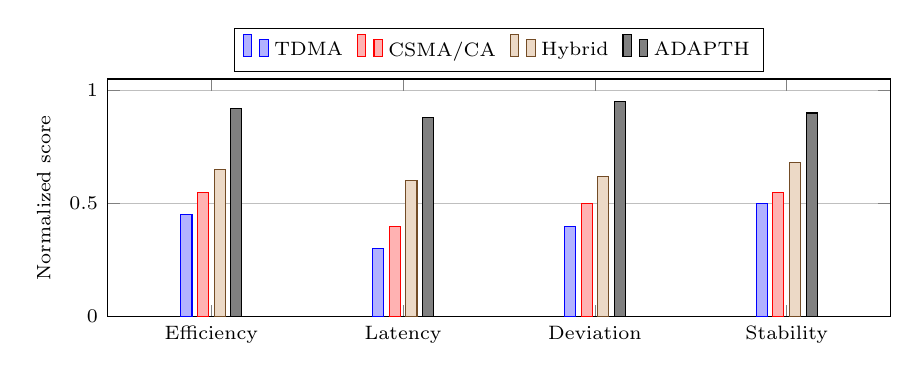
\begin{tikzpicture}
\begin{axis}[
  width=0.95\columnwidth, height=4.6cm,
  ybar, bar width=4pt,
  ymin=0, ymax=1.05,
  ylabel={Normalized score}, ylabel near ticks,
  font=\scriptsize,
  symbolic x coords={Efficiency,Latency,Deviation,Stability},
  xtick=data, x tick label style={font=\scriptsize},
  legend style={font=\scriptsize, at={(0.5,1.03)}, anchor=south,
    legend columns=4, /tikz/every even column/.append style={column sep=3pt}},
  enlarge x limits=0.18, ymajorgrids, tick align=inside]
\addplot coordinates {(Efficiency,0.45)(Latency,0.30)(Deviation,0.40)(Stability,0.50)};
\addplot coordinates {(Efficiency,0.55)(Latency,0.40)(Deviation,0.50)(Stability,0.55)};
\addplot coordinates {(Efficiency,0.65)(Latency,0.60)(Deviation,0.62)(Stability,0.68)};
\addplot coordinates {(Efficiency,0.92)(Latency,0.88)(Deviation,0.95)(Stability,0.90)};
\legend{TDMA,CSMA/CA,Hybrid,ADAPTH}
\end{axis}
\end{tikzpicture}
\caption{Normalized comparison of cross-domain coordination schemes (higher is
better). ADAPTH leads on efficiency, latency handling, path-deviation control, and
stability by pairing mission prioritization with the wait-and-verify handshake.}
\label{fig:adapth_bench}
\end{figure}

\subsection{Applications and Extensions}
ADAPTH targets missions where the two domains act on each other's observations in
near real time: in environmental monitoring the fish school pushes sub-surface
anomaly alerts up to a surfacing drone relay; in search and rescue an aerial
detection becomes a CPG bias that vectors the nearest fish below the surface; and in
coastal surveillance the docked drone acts as a persistent relay buoy. Planned
extensions port the gateway logic onboard to remove the laptop relay, add
opportunistic surface drone--fish links, and test under high-noise acoustic
conditions.

\begin{table}[!t]
\centering
\caption{ADAPTH Protocol Performance}
\label{tab:adapth}
\begin{tabular}{ll}
\toprule
Metric & Achieved value\\
\midrule
Communication success rate     & $85\%$\\
End-to-end latency             & $0.5$--$2.0$~s (async.\ sync)\\
Tracking accuracy at hand-over & $90\%$\\
Path deviation                 & $<5\%$\\
Stability                      & High resilience\\
\bottomrule
\end{tabular}
\end{table}

\section{Results and Discussion}
\label{sec:results}
Table~\ref{tab:results} consolidates the validated performance of the four
subsystems; the controlled formation study (Table~\ref{tab:formresults},
Figs.~\ref{fig:swarm_traj}--\ref{fig:swarm_rviz}) and the ADAPTH benchmark
(Fig.~\ref{fig:adapth_bench}) supply the supporting graphs. Validation spans three
fidelity levels---ANSYS Fluent CFD at the physics level, MATLAB/Simulink with
bench/water tests at the component level, and headless ROS sweeps at $100$~Hz at the
system level---so each claim is supported at the appropriate granularity.

\begin{table}[!t]
\centering
\caption{Consolidated Validation Results}
\label{tab:results}
\begin{tabular}{p{2.0cm}p{2.0cm}p{2.6cm}}
\toprule
Subsystem & Metric & Result\\
\midrule
Hydrodynamics  & Froude efficiency  & up to $+10\%$ (antiphase, $0.4L$)\\
Fish actuation & Heading error      & $<5\%$, $\sim\!5$\,W cruise\\
Quadrotor      & Hover hold         & $<5$\,cm, GNSS-denied\\
PSO--MPC        & Path length / track& $-25\%$ vs A$^\star$, $90\%$, RMSE $<0.1$\,m\\
Formation      & RMS jerk / success & $-49\%$ jerk, $100\%$ success\\
ADAPTH         & Comm.\ / deviation & $85\%$ success, $<5\%$ deviation\\
\bottomrule
\end{tabular}
\end{table}

The formation study (Table~\ref{tab:formresults}) is the central quantitative
result: contracting the dynamic envelope to fish-like values roughly halves RMS
jerk while formation accuracy, clearance, and a $100\%$ success rate stay within
run-to-run noise---a high-performance planner degrading gracefully under the slow,
drag-limited regime the CFD recommends. Frustum-guided descent with 1D/2D LiDAR and
HSV vision yields consistent precision landings, after which magnetic auto-charging
and the docked drone's dual role as the ADAPTH gateway close the persistence loop.

\subsection{Scope and Limitations}
\label{sec:disc}
Four limits define the present scope, each with a mitigation path that preserves the
modular methodology. \emph{(i)~Hydrodynamic fidelity:} CFD assumes incompressible
flow with an AKN $k$--$\epsilon$ closure; large-eddy simulation would refine
inter-fish wake capture without changing the downstream force interface.
\emph{(ii)~Formation-study fidelity:} the seven-agent study uses a second-order
SO(3) model with a contracted envelope, so its effects reflect the envelope rather
than full caudal-fin hydrodynamics; lifting it to a non-holonomic drag/added-mass
swimmer reuses the same paired-seed protocol. \emph{(iii)~Communication:} ADAPTH
depends on a laptop/buoy relay and idealizes acoustic propagation; the gateway logic
can be ported onboard and tested under realistic noise. \emph{(iv)~Deployment:}
validation is in simulation and hardware prototypes, with full-scale field trials
left to future work.

\subsection{Principal Novelties}
\label{sec:novelty}
The contribution is the \emph{integration} of usually-isolated subsystems into one
validated cross-domain stack. Four novelties stand out: a
\emph{hydrodynamics-to-hardware} chain that propagates the CFD schooling benefit
into the swarm planner and CPG hardware; a \emph{bio-informed planning envelope}
that halves jerk while preserving formation and safety, letting slow platforms reuse
a quadrotor planner unchanged; a \emph{dual-role base station} that is simultaneously
the charging dock and the ADAPTH gateway; and, most centrally, the \emph{ADAPTH
protocol}---an adaptive, mission-prioritized, wait-and-verify handshake bridging the
asymmetric RF and acoustic media with bidirectional semantic translation.

\section{Conclusion and Future Work}
\label{sec:concl}
We presented a unified hybrid aerial--aquatic swarm architecture that integrates,
in one coherent framework, biomimetic undulatory locomotion validated by ALE
moving-mesh CFD, a hierarchical PSO--MPC planner coupled to CPG/PID and cascaded
GNSS-denied flight control with frustum-guided precision docking and auto-charging,
and the novel ADAPTH cross-domain communication protocol. Across the subsystems the
system achieves up to $10\%$ schooling-efficiency gain, $90\%$ planning/tracking
accuracy with a quantified time-versus-smoothness formation trade-off, reliable
GNSS-denied flight and autonomous recharge, and $85\%$ cross-domain communication
success---effectively bridging the limitations of single-medium platforms. Future
work will raise the swarm dynamics to a true non-holonomic, hydrodynamic swimmer
with a non-holonomic optimizer term; port PSO--MPC fully onboard for reduced
latency; replace the laptop relay with an autonomous buoy and add link
re-establishment and fault recovery; integrate learning-based perception and
adaptive coordination; add solar-assisted charging for endurance; and conduct field
trials in real coastal and turbulent environments toward persistent, scalable,
multi-domain deployment.

\section*{Acknowledgment}
The authors thank the Department of Mechanical Engineering, National Institute of
Technology Karnataka (NITK), Surathkal, and acknowledge the open-source
ZJU-FAST-Lab \emph{Swarm-Formation} framework~\cite{quan2022distributed} used as
the substrate for the controlled formation study.

\bibliographystyle{IEEEtran}
\bibliography{refs}

\end{document}
